\documentclass[openany]{book}
\author{Bryan Wolfford}
\title{GPGPU Accelerated Iterative Filtering of Scalar Fields on Discrete Manifolds}
\date{\today}
%
\usepackage{syntonly}
%\syntaxonly
\usepackage{amsmath}
\usepackage{tikz}
\usepackage{graphicx}
%\usepackage[lofdepth,lotdepth]{subfig}
\usepackage[colorinlistoftodos]{todonotes}
\usepackage{makeidx}
\usepackage[intoc]{nomencl}
\usepackage{multicol}
\usepackage[numbib,numindex]{tocbibind}
\usepackage[font=small,labelfont=bf,labelsep=period,justification=centerlast]{caption}
\usepackage{subcaption}
\usepackage{floatrow}
\usepackage{parskip}
\usepackage[linesnumbered,ruled]{algorithm2e}
\usepackage[bookmarks,colorlinks]{hyperref}
\hypersetup{colorlinks,
	citecolor=[rgb]{0,0,0.5},
	filecolor=[rgb]{0,0,0.5},
	linkcolor=[rgb]{0,0,0.5},
	urlcolor=[rgb]{0,0,0.5},
	pdfinfo={
		Author={Bryan Wolfford},
		Title={GPGPU Accelerated Iterative Filtering of Scalar Fields on Discrete Manifolds},
	}
}
%For nomenclature 2 columns
\renewcommand*{\nompreamble}{\begin{multicols}{2}}
\renewcommand*{\nompostamble}{\end{multicols}}
\setlength{\columnsep}{2em}
%\setlength{\nomitemsep}{-\parsep}
%\renewcommand{\nomunit}{\dotfill}
\renewcommand{\nomgroup}[1]{%
	\item[]\hspace*{-\leftmargin}%
	\rule[2pt]{0.45\linewidth}{1pt}%
	\hfill #1\hfill%
	\rule[2pt]{0.45\linewidth}{1pt}
}
%
\newcommand{\bc}{\mathbf{c}}
\newcommand{\bp}{\mathbf{p}}
\newcommand{\bs}{\mathbf{s}}
\newcommand{\bt}{\mathbf{t}}
\newcommand{\bG}{\mathcal{\Gamma}}
\newcommand{\bM}{\mathcal{M}}
\newcommand{\bN}{\mathcal{N}}
\newcommand{\Dc}{\Delta c}
\newcommand{\Dm}{\Delta_\text{min}}
\newcommand{\gDm}{\overline{\Dm}}
\newcommand{\Dz}{\Delta\zeta}
\newcommand{\sipo}{i\kern-.7pt\scalebox{0.66}{+}\kern-1.2pt1}
%
\newcommand{\igHalfWidth}{0.48\linewidth}
%TODO:why can"t I use this as an option for includegraphics?
%
\newcommand{\todoRemove}[1]{\todo[color=red!40]{#1}}
\newcommand{\todoCitation}[1]{\todo[color=teal!40]{citation required}}
\newcommand{\todoResearch}[1]{\todo[color=cyan!40]{#1}}
\newcommand{\todoElaborate}[1]{\todo[color=violet!40]{#1}}
\newcommand{\todoReword}[1]{\todo[color=magenta!40]{#1}}
\newcommand{\todoStyle}[1]{\todo[color=pink!40]{#1}}
%xcolor base colors:
%	black
%	blue
%	brown
%%%	cyan
%	lime
%%%	magenta
%	olive
%	orange
%%%	pink
%	purple
%%%	red
%%%	teal
%%%	violet
%	white
%	yellow
%
\includeonly{
	chapters/0-Front-matter,
%	chapters/1-Introduction-Motivation,
%	chapters/2-Background,
%	chapters/3-Related-Work,
	chapters/4-One-Ring-Filter,
%	chapters/5-Profiling-Exploiting-Concurrency,
%	chapters/6-Meat-3,
%	chapters/7-Experiments-Evaluation,
%	chapters/8-Distribution,
%	chapters/9-Conclusion,
%	chapters/A1-Appendix,
%	chapters/A2-Appendix,
%	chapters/Z1-Back-Matter
}
%
\makeindex
\makenomenclature
\begin{document}
\include{chapters/0-Front-matter}
%
\mainmatter
\chapter{Introduction \& Motivation}
\section{3D Data is important (and big).}
Lorem ipsum dolor sit amet, consectetur adipiscing elit. Morbi tincidunt eget 
ipsum eu iaculis. Cras vel sem eu velit eleifend porta vel sit amet massa. Etiam 
a posuere nunc. Aenean aliquam viverra dapibus. Aliquam ac eros a purus feugiat 
rhoncus. Donec faucibus ut nibh ut cursus. Aliquam erat volutpat. Proin efficitur 
nulla sit amet iaculis condimentum. Cras placerat leo vitae venenatis feugiat. In 
hac habitasse platea dictumst. Orci varius natoque penatibus et magnis dis 
parturient montes, nascetur ridiculus mus. In aliquet sagittis dui eu pulvinar. 
Morbi a arcu eu dolor sagittis varius. Aliquam dignissim tortor sed tortor 
suscipit, eget imperdiet mauris convallis.~\cite[p.~00]{todoCitation}\todoCitation


\section{Serial is slow.}
Lorem ipsum dolor sit amet, consectetur adipiscing elit. Morbi tincidunt eget 
ipsum eu iaculis. Cras vel sem eu velit eleifend porta vel sit amet massa. Etiam 
a posuere nunc. Aenean aliquam viverra dapibus. Aliquam ac eros a purus feugiat 
rhoncus. Donec faucibus ut nibh ut cursus. Aliquam erat volutpat. Proin efficitur 
nulla sit amet iaculis condimentum. Cras placerat leo vitae venenatis feugiat. In 
hac habitasse platea dictumst. Orci varius natoque penatibus et magnis dis 
parturient montes, nascetur ridiculus mus. In aliquet sagittis dui eu pulvinar. 
Morbi a arcu eu dolor sagittis varius. Aliquam dignissim tortor sed tortor 
suscipit, eget imperdiet mauris convallis.~\cite[p.~00]{todoCitation}\todoCitation



\section{Concurrency is fast.}
Lorem ipsum dolor sit amet, consectetur adipiscing elit. Morbi tincidunt eget 
ipsum eu iaculis. Cras vel sem eu velit eleifend porta vel sit amet massa. Etiam 
a posuere nunc. Aenean aliquam viverra dapibus. Aliquam ac eros a purus feugiat 
rhoncus. Donec faucibus ut nibh ut cursus. Aliquam erat volutpat. Proin efficitur 
nulla sit amet iaculis condimentum. Cras placerat leo vitae venenatis feugiat. In 
hac habitasse platea dictumst. Orci varius natoque penatibus et magnis dis 
parturient montes, nascetur ridiculus mus. In aliquet sagittis dui eu pulvinar. 
Morbi a arcu eu dolor sagittis varius. Aliquam dignissim tortor sed tortor 
suscipit, eget imperdiet mauris convallis.~\cite[p.~00]{todoCitation}\todoCitation



\section{GPUs are commercially available, use to exploit concurrency.}
Lorem ipsum dolor sit amet, consectetur adipiscing elit. Morbi tincidunt eget 
ipsum eu iaculis. Cras vel sem eu velit eleifend porta vel sit amet massa. Etiam 
a posuere nunc. Aenean aliquam viverra dapibus. Aliquam ac eros a purus feugiat 
rhoncus. Donec faucibus ut nibh ut cursus. Aliquam erat volutpat. Proin efficitur 
nulla sit amet iaculis condimentum. Cras placerat leo vitae venenatis feugiat. In 
hac habitasse platea dictumst. Orci varius natoque penatibus et magnis dis 
parturient montes, nascetur ridiculus mus. In aliquet sagittis dui eu pulvinar. 
Morbi a arcu eu dolor sagittis varius. Aliquam dignissim tortor sed tortor 
suscipit, eget imperdiet mauris convallis.~\cite[p.~00]{todoCitation}\todoCitation



\section{Noise propagates when processing dense meshes}
When the field of function values $f(\bp_i)$ are rendered as isolines, or when one visualizes connected components of segmented areas of interest.

In dense, high-resolution meshes, which can feature several hundred points per mm$^2$~\cite[p.~00]{todoCitation}\todoCitation, one can see noise propagating within the results of the MSII filter as jagged outlines.~\cite[s.~3.2]{Mara17}

The design principles for filtering of function 
values in irregular grids are the same as for those well-known algorithms used 
for raster images. However, they require adaptation as there is no fixed 
distance between the points and no fixed number of neighboring points in 
1-rings of irregular grids.~\cite[s.~3.2]{Mara17}



\section{Structure of this paper}
This paper is structed as follows:
1. 3D data acquisition
2. noise filtering
3. GPGPUs, parallel processing, concurrency profiling
4. the published and current fast 1-ring smoothing filters
5. how we exploit found concurrency
6. experiments and mesh generators
7. compare serial vs parallel results and compute times

\chapter{Background}
\section{3DData}
\subsection{Synthetic vs Aquired 3D Meshes}
We have to mention that a common misunderstanding is that acquired 3D-objects
are similar or even identical to modeled 3D-objects – this is not true! 
Both utilize the same methods for organizing the data, but per-se the concepts 
of primitives and other simplifications do not exist for acquired 3D-objects. 
Additionally acquired 3D-objects contain noise, which partially prevents 
simplification. Furthermore this adds to the complexity as simple objects, 
which can be modeled with a few primitives, are acquired as pointclouds, which 
can – and do – have thousands to millions of points. For worst cases even the 
assumption of a non-manifold mesh3 may not apply due to incorrect registration 
of multiple 3D-scans [BR07]. As we know from our previous work, there is always 
at least a minor number of non-manifold points within our data, which has to be 
taken care of to achieve a robust system [Mar06]. Reducing the resolution for 
acquisition contradicts with the Shannon theorem, while the rule of thumb from 
our previous projects is: the resolution for acquisition has to be 5 times the 
size of the smallest detail to be acquired.~\cite[p.~25]{Mara12}

\subsection{3DData}
Virtually all the software packages accompanying 3D-scanners export
a 2D-non-planar, manifold and non-regular surface mesh consisting of vertices 
connected as triangles, and having an optional texture map. This kind of a
surface mesh is often and shortly called 3D-data by Computer Vision (CV) [BB82]
groups. In the field of geography a similar data structure is called
Triangulated Irregular Networks (TINs), which also can be acquired with
non-optical methods (e.g. LIDAR). As for our test-case the cuneiform script is
generally defined by pure geometry and the consideration of a texture-map is
per-se not necessary.~\cite[p.~25]{Mara12}

\subsection{Points}
The most primitive element of our data is a measuring point p, having three 
Cartesian coordinates x, y and z. In Computer Graphics and Computer Vision these 
points are called vertices, while they are called position vectors in R 3 in 
Linear Algebra (LA). As generally all vertices are unique and in no particular 
order, we address them by the index i and store them as a list L v :
L v = { p 1 , . . . , p i , . . . , p i max } with i max = ∣L v ∣ and i = Z + ∧ 
i ≤ i max (2.1)
The indexing in Equation 2.1 corresponds to the usage of 1 to address the first 
element of a list. Alternatively the first element can also be addressed using 0 
to address the first element of a data structure in programming languages like 
C/C++: i = Z + 0 ∧ i < i max . For compliance with textbook mathematics we use 1 
to address the first element of a data structure, vector, etc. for all other 
equations. 3 A mesh having more than two triangles connected by one edge. 25∣L v 
∣ is the cardinality of the list of vertices, while ∣p i ∣ is the length of the 
position vector.
In case of position vector, its length is equal
√ to the distance of a vertex from the origin
T
o = (0, 0, 0) of the coordinate system: x 2 i + y i 2 + z i 2 . These position 
vectors sampling the surface M 2 in R 3 are identified within homogeneous 
coordinate system [Gra30] having
w i = 1 as fourth coordinate~\cite[p.~25-26]{Mara12}

\subsection{Faces}
Counte-Clokwise vs CloCkwise~\cite[p.~00]{todoCitation}\todoCitation
The second important class of primitive elements are the so-called faces, which 
are triangles t having an orientation provided by the data-structure of the 
3D-models, e.g. for visualization using virtual illumination. The triangles are 
addressed using the index j,while each triangle has three implicit edges: e a j 
, e b j and e c j .t j ∶= {p A j , p B j , p C j } ≡ {A j , B j , C j }p C jyyyy
yyyye bjp A je cjt = {A, B, C}abbreviated:EE eEE ajEEEEp B j~~~~~~ ~bA(2.4)C \_ 
The faces are stored in the list L f : L f = { t 1 , . . . , t j , . . . , t j 
max } with j max = ∣L f ∣ and j = Z + ∧ j ≤ j max
(2.5)
So the list of vertices L v and the list of faces L f describe the discrete, 
meshed geometry of the surface M 2 as provided by our 3D-models (triangulation 
networks): M 2 ∶= L M = {L v , L f } (2.6)
This basic list L M will be extended by other surface properties (e.g. color) in 
the following sections and chapters. In case no L f is provided, it is a 
necessity to perform a point set triangulation [BE92, HK09] to compute L f from 
L v .~\cite[p.~26]{Mara12}

\subsection{Funtion Values}
Lorem ipsum dolor sit amet, consectetur adipiscing elit. Morbi tincidunt eget 
ipsum eu iaculis. Cras vel sem eu velit eleifend porta vel sit amet massa. Etiam 
a posuere nunc. Aenean aliquam viverra dapibus. Aliquam ac eros a purus feugiat 
rhoncus. Donec faucibus ut nibh ut cursus. Aliquam erat volutpat. Proin efficitur 
nulla sit amet iaculis condimentum. Cras placerat leo vitae venenatis feugiat. In 
hac habitasse platea dictumst. Orci varius natoque penatibus et magnis dis 
parturient montes, nascetur ridiculus mus. In aliquet sagittis dui eu pulvinar. 
Morbi a arcu eu dolor sagittis varius. Aliquam dignissim tortor sed tortor 
suscipit, eget imperdiet mauris convallis.~\cite[p.~00]{todoCitation}\todoCitation


%\section{Irregular Non-Manifold Meshes and 2D-Manifolds in 3D-Space}
\subsection{Treatment of Unclean Data}
%\subsection{Borders and Edges}
Proper detection and treatment of borders of M 2 is important even for watertight
3D-models as we will encounter borders for subsets M 2 in Chapter 4. These 
subsets are typically connected components also called labeled regions – see 
Chapter 2 in [BB82]. In general we have to expect holes within the surfaces of 
our 3D-models, because the data structure is designed to handle real world data, 
where measurements of the surface may be missing.
Holes within the surfaces of a 3D-model mean mathematically, that M 2 can have 
one or more borders. Consequently there is an area along the borders, which have 
to be determined. Borders have to be treated differently than the rest of the 
surface. The border area contains faces with vertices, which can be computed by 
examination of theedges e of t. A list of orientated edges L e can be derived 
from L f by splitting each triple
{j A , j B , j C } into three tuples:
t j ↦ L e j (t j ) = {{A j , B j }, {B j , C j }, {C j , A j }} ≡ {e c j , 
e b j , e a j }
L e = { e c 1 , e b 1 , e a 1 , . . . , e c jmax , e b jmax , e a jmax }
⇒ ∣L e ∣ = 3∣L f ∣ , with k = Z + ∧ k ≤ k max ∧ k max = 3j max we get:
L e = { e 1 , e 2 , e 3 , . . . , e k max −2 , e k max −1 , e k max }
(2.13)(2.14)(2.15)
Edges not on the border appear twice within a mesh with inverted orientation. 
An edge e m = {A m , B m } is on the border ∂M 2 of M 2 , when: ∄ k with e k = 
{B m , A m } ∈ L e (2.16)
These edges are stored in the list L ∂e , which holds the indices of edges along 
the boundary of the mesh. A mesh with an empty list of edges L ∂e = Ø is called 
a closed mesh.Consequently the face t k−(k mod 3) and the vertices p A m and p B 
m are on the border, 3
when M 2 is a manifold. The only exceptions are the so-called solo vertices, 
which are not connected to any face. These vertices are extreme cases of holes 
and typically occur as outliers for surfaces with properties like translucency, 
high reflectance and/or dark color. Let I be an index set for solo vertices, the 
list of solo vertices L v s is be determined by:
L v s ∶= {p s ∣ ∄ t j ∈ L f with
t j = {A j = s, B j , C j }∨
t j = {A j , B j = s, C j }∨
t j = {A j , B j , C j = s}} s∈I ⊆ L v
(2.17)(2.18)(2.19)(2.20)
When L f = Ø than L v s = L v , which is the definition of a point cloud. This 
is the contrary of an ideal M 2 having L v s = Ø as a necessary 
criteria.~\cite[p.~28]{Mara12}

%\subsection{Adjacencies, Singularities and k-ring Neighborhoods}
Knowing the neighbors of a measuring point is the key to analyze our data. 
For regular data structures, e.g. 2D-images a pixel has four neighbors in 
orthogonal direction with a (relative) geometric distance of 1 and four further 
neighbors with a geometric distance of √2. Neglecting the geometric distance we 
can apply the same for vertices and faces and determine their neighbors using 
the orientation of the triangles:
• A face t j is adjacent to a face t i , when t j has an edge e m = {A m , B m } 
and t i has an edge e k = {B m , A m }.
• The vertices adjacent to a vertex p i are those p̊ i , belonging to the
faces t̊ i ∶= {A i , B ≠i , C ≠i } ∨ {A ≠i , B i , C ≠i } ∨ {A ≠i , B ≠i , C i }.
Faces t̊ i and vertices p̊ i belong to the so-called 1-ring as they have 
distance of 1 within the graph of the mesh. The 1-ring can be extended to a 
2-ring by using the verticesp̊ i as p i , which adds vertices and faces having 
a distance of 2 within the graph. This iterative concept can be repeated k times 
and the neighborhood is than refered to as k-ring. The distance within the graph 
can not be assumed equal to the geometric distance nor geodesic distance. 
However it is used throughout literature as experiments are often done on 
synthetic data – especially in the field of Computer Graphics. Figure 2.6 shows 
the scheme of the 1-ring and an example for a 5-ring on a synthetic sphere in 
contrast to 5-rings on an acquired mesh. Even the triangles of the sphere are 
almost equal, we see that the outlines of the k-rings have a hexagonal shape, 
while geodesic ring would have the shape of a circle. Already the 1-rings of 
the acquired mesh have completely arbitrary shapes and sizes.
(a)(b)(c)(d)
Figure 2.6: k-ring neighborhood: (a) Scheme of a 1-ring neighborhood and 1 to 
5-ring neighborhood for (b) a synthetic sphere and (c) for a wedge acquired 
using a 3D-scanner. The 1-ring shown in Figure 2.6a is closely related to the 
so-called triangle-fan used by Open Graphics Language (OpenGL). While the 
Figure represents the most common case of an 1-ring equal to a triangle-fan as 
most parts of M 2 are organized like this. The second common case looks the 
same, with one or more adjacent faces missing – this is the case, when p̊ i is 
on the border of the mesh. However the data structure allows that non-adjacent 
faces are missing leading to singular vertices – not to be confused with solo 
vertices. 29 We can identify singular vertices connecting different parts of M 
2 by determining one triangle-fan per vertex and compare them to the 1-ring 
neighborhood. The faces of the 1-ring are determined just by the presence of a 
shared central vertex [MB05] as shown before. Having the 1-ring we need to test 
if we can walk around the shared vertex using the faces and their neighbors. 
This is shown in Figure 2.7a, where we can start at any of the vertices 
{B, . . . , G} following the directional edges between them. We than will 
arrive at vertex p G . If we have not started at p B , we will have to 
backtrack the edges in opposite direction as p A is a vertex on the border 
∂M 2 . In the end we will have visited all vertices of the triangle fan 
{B, . . . , G}. When p A is not on the border, because a triangle {A, G, B} 
exists, we can visit all vertices without backtracking. Figure 2.7b shows the 
scheme for a border vertex, which is singular, because we can visit either the 
{B, C, D, E} or {F, G, H} of these two triangle-fans. Figure 2.7c shows an 
example from a 3D-model, where a non-border, singular vertex p A connects 
different parts of the mesh.
(a)(b)(C)
Figure 2.7: Schematic visualization of (a) a non-singular vertex p A with its 
triangle fan equaling its 1-ring neighborhood. When there is a triangle 
{A, G, B} the fan is closed – if not p A , p B and p G are vertices on the 
border of M 2 . (b) Singular vertex p A connecting two triangle fans.
(c) Real world example for a singular vertex p A .~\cite[p.~29]{Mara12}

%\subsection{Non-Manifold Edges}
Previous Sections have shown that 3D-models from optical 3D-scanners consist of a dis-
crete surface representation and are generally not regular having singular vertices due to
the missing constraints from file formats organized by L v and L f . The lack of these con-
straints also allows for non-manifold structures as faces can have more than one neighbor
per edge. This is useful for synthetic 3D-models from Computer Aided Design (CAD)
systems, e.g to connect primitives like walls of buildings. However these non-manifold
structures have to be detected and treated. Methods to analyze 3D-data have to search
along the graph of the mesh. Applying e.g. a search algorithm designed for manifold
30surfaces may not reach all parts of the mesh as it will ignore junctions caused by non-
manifoldness. In worst-case scenarios an algorithm may be trapped in an infinite loop. By
definition of our data structure, non-manifold edges, singular vertices and agglutinated
faces can occur.
Manifold edges are edges shared by exactly two faces. Exceptions are edges at the
border of the surface, having no adjacent face. As each edge derived from L f has an
orientation, a non-manifold edge e 2+
m is found, when there are two edges from different
triangles defined by the same vertices, having the same direction:e 2+
m ∶= e k ∈ t u ∨ e m ∈ t v ∨ e k = e m = {A m , B m }(2.21)
Such a non-manifold edge can connect an arbitrary number of faces t ≠v , which leads to:
e + m ∶= e ≠m ∈ t ≠v ∨ e m ∈ t v ∨ ∀e ≠m ∶ e ≠m = e m = {A m , B m }(2.22)
As the faces t have an orientation, a special case of wrong connections can be found
using the above definition: pairs of faces sharing one edge having the edge orientated in
the same direction. This means that one of the faces has a wrong orientation resulting
in a normal vector pointing in the negative direction. Such cases become immediately
visible, when rendered using a virtual illumination and have to be removed or corrected.
Figure 2.8a shows the scheme for one edge e k≠m connecting two manifold faces (t u , t v ).
Figure 2.8b shows the same faces having a face t w added sharing a non-manifold edge
e k=m and Figure 2.8c shows the special case for a manifold edge connecting the face t w
having a wrong orientation.(a)(b)(c)
Figure 2.8: Schematic visualization of M 2 in green with an edge connecting (a) two manifold
faces (t u , t v ) and (b) the face t w added along the non-manifold edge e k = e m and 
(c) having aface t w embedded with a wrong orientation.~\cite[p.~30-31]{Mara12}

%\subsection{Agglutinated Faces and Faces with Zero Area}
Faces literally sticking together having a proper orientation (no e + ) are typical remains
of outliers from acquisition. They can be removed as they describe parts of objects
without any volume. This can be shown using Equation 2.10 with two faces sharing
the same vertices in opposite orientation. Let the first face be t 1 ∶= {p a , p b , p c } and the
agglutination face be t 2 ∶= {p c , p b , p a }, we can simplify: s = s 1 = s 2 , A(t) = 
A(t 1 ) = A(t 2 ) and n̂ 2 = −n̂ 1 and substitute:⎛ s x 1 ⎞⎛ s x 2 ⎞⎛ s x ⎞
V M = A(t 1 ) ⎜ 0 ⎟ n̂ 1 + A(t 2 ) ⎜ 0 ⎟ n̂ 2 = A(t) ⎜ 0 ⎟ (n̂ 1 − n̂ 1 ) = 0⎝ 0 ⎠⎝ 0 ⎠⎝ 0 ⎠(2.23)
An indicator for an agglutinated face are edges with faces having a wrong orientation as
shown in Figure 2.8c. In practical examples agglunating faces often appear along non-
manifold edges. However agglunating faces can be found and removed using the following
definition, which should be done before removing non-manifold edges and removing faces
with wrong orientation to minimize the changes to the mesh.
∃ t i ∨t j ∈ L f with t i ∶= {A i , B i , C i } and t j ∶= {C i , B i , A i }∧
{B i , A i , C i }∧{A i , C i , B i } (2.24)
Besides agglutinated faces having enclosing no volume, there also exist degenerated
faces having no area. This happens, when two or all three vertices of a face have the same
position vector. For example, when we substitue p A = p B in Equation 2.7 we get:
n j = (p B j − p B j ) × (p C j − p B j ) = (0, 0, 0) T and therefore A(t j ) =
∣n j ∣= 02(2.25)
Summarizing this Section we can detect the worst case scenarios within the data
structure of files provided by 3D-scanners, which can render an algorithm for local surface
filtering instable, because of e.g. an area of zero leading to a division by zero. The case
of self-intersecting surfaces as known from synthetic data and their treatment [JSC04] is
not necessary, as it does not change or influence the critical surfaces properties in respect
to the methods presented within this thesis.~\cite[p.~32]{Mara12}

%\section{Data cleaning - Ensuring a Perfect Mesh} 
%IS THIS STILL NECCESSARY? Since, Filtering can handle edges
How does the filter handle edges and unclean meshes?

The modular processing pipeline allows for adaption of the workflow for feature 
extraction depending on the application. As modules like the MSII filter 
provides several variants to compute integral invariants leads to a large number 
of combinations. Hard-coding all these combinations is as impracticable as 
asking an user to implement their own pipeline. The compromise is to provide an 
user interface including visualization of intermediate results.
Therefore GigaMesh got a base layer of classes and methods as described 
previously, which can be used to assemble a tool-chain for command line use on 
compute servers. To give a visual feedback of final and intermediate results an 
OpenGL layer was added. On top of this second layer a GUI using Trolltech’s Qt, 
because it is available on all major platforms under the GNU General Public 
License (GPL) – an Open Source license.

Layer I: Processing Methods
This layer contains all the algorithms to compute integral invariants as well as 
means to determine irregularities shown in Section 2.2. In spite of the integral 
invariant algorithms being robust against irregularities and missing data 
(holes), the results improve, when faulty parts of a mesh are repaired. A mesh is 
typically repaired in a first step by removing faulty primitives.
Removing primitives of a mesh is related to the morphological operation erosion. 
Section 2.2 on pages 25ff. shows different types primitives to be eroded, because 
they are considered irregular. Each type of irregularity requires a different 
erosion method. The application of an erosion method can introduce new 
irregularities e.g. removing a nonmanifold edge can lead to a singular vertex. 
Another common case is the removal of such singular vertices, which leads to new 
singular vertices within the 1-ring neighborhood. This means that the erosion 
methods have to be applied repeatingly and their order has an influence on the 
amount of removed primitives. As this number has to be kept to a minimum the 
Layer I of GigaMesh provides an highly automated mesh polishing algorithm, which 
fulfills this demand. Erosion additional leads to a segmentation of the mesh M2 
into connected components C, which are either a meaningful part of the object or 
noise. The parts introduced by measuring errors are typically smaller than the 
meaningful components.
Therefore the connected components labeling as shown in Section 4.1.1 on pages 
94ff. is applied and the surface area ∣Cl ∣ of each connected Cl is computed. 
Then the components are sorted by their area: ∣C1∣ ≤ ∣C2∣ ≤ ⋅ ⋅ ⋅ ≤ ∣Cn∣ (4.29) 
Next the index i is determined as there typically exists: ∣Ci ∣ ⋘ ∣Ci+1∣ (4.30) 
120 and leads to a threshold tC > ∣Ci ∣ to remove small surface components 
introduced by noise, which are shortly denoted as labels Ci<t .
Removing singular vertices has to applied before removing Ci<t , because the 
erosion of singularities typically increases the number of labels Ci<t . The 
same can happen, when faces along non-manifold edges are removed. Before these 
are removed, sticky faces have be removed as very first, because they introduce 
a sub-set of non-manifold edges. This leads to a sequence of erosion operations, 
which has to be repeated until the number of vertices ∣Lv∣ and faces ∣Lf ∣ of a 
3D-model does not decrease anymore:
1. Remove sticky faces and face with zero area shown on page 32.
2. Remove non-manifold faces shown on page 30.
3. Label all vertices as shown using Algorithm 12 on page 95 ↝ {. . . , Cl , . 
. . } ∧ ∄CØ without considering the function value f(pi), e.g. using tp = +∞.
4. Compute the area ∣Cl ∣ of all labels Cl using Equation 2.7 on page 27.
5. Remove all labels Ci<t having an area less than tC.
6. Remove solo vertices Lvs shown in Equation 2.20 on page 28.
7. Remove singular vertices – shown on page 29.
Afterwards the eroded mesh becomes a so-called clean mesh. Note that in most of 
the cases of clean meshes, there will be holes ∂M2. Therefore these holes have 
to be filled, which can be achieved by dilation as shown in [Lie03]. Due to 
numeric errors the dilation can re-introduce faces with zero area and other 
irregularities, the erosion and dilation have to be repeatingly applied to a mesh 
until no more holes are present:
1. Erode the mesh until it is clean as shown above.
2. Determine a list of boundaries ∂M2 ∶= n ⋃ i=1 ∂Ci of the holes.
3. Remove boundaries ∂Ci of large connected components with ∣Ci ∣ > tC from the 
list.
4. Fill the remaining holes ∂Ci>t within the list.
The result is a so-called perfect mesh, which provides the best numeric results 
in respect to the quality of an acquired data-set. Because even a perfect mesh 
will have boundaries ∂M2 the border treatment of the algorithms to compute 
integral invariants stays relevant for robust processing. However, when obeying 
the described order, it is guaranteed that the remaining boundaries are kept as 
far as possible from the areas of interest.~\cite[p.~120]{Mara12}



\section{Achitectures of Concurrency}
Serial vs Multi-threaded vs GPU order from slow to fast.~\cite[p.~00]{todoCitation}\todoCitation



\section{What is CUDA?}
Graphical Processor Units, GPUs, are highly parallel, multithreaded, manycore 
processors typically characterized by very high computational power and 
tremendous memory bandwidth. A GPU is especially well-suited when used to 
data-parallel computations, in which the same program is executed on many data 
elements in parallel.~\cite[p.~1.1]{CUDA18}

Mainstream processor chips, both CPU and GPUs, are now parallel systems, and as 
this parallelism continues to scale with Moore's law, the real challenge is to 
develop application software that transparently scales its parallelism to 
leverage the increasing number of processor cores. The CUDA parallel 
programming model, introduced by NVIDIA in November of 2006, was specifically 
designed to overcome this challenge.~\cite[p.~1.3]{CUDA18}

In fact, due to its inherent scalable programming model in which problems are 
decomposed in a way that each block of thread\index{thread} can be scheduled on 
any of the available multiprocessors within a GPU, in any order, concurrently 
or sequentially, so that any compiled CUDA program, such as our implementation 
of the MSII filter, can be executed on any number of multiprocessors, and only 
the runtime system needs to know the physical multiprocessor 
count.~\cite[p.~1.3]{CUDA18}

~~~~~~~~~

CUDA C extends C by allowing the programmer to define C functions, called 
kernels, that, when called, are executed N times in parallel by N different 
CUDA thread\index{thread}, as opposed to only once like regular C 
functions.~\cite[p.~2.1]{CUDA18}

thread\index{thread} can be identified using a one-dimensional, 
two-dimensional, or three-dimensional thread\index{thread} index, forming a 
one-dimensional, two-dimensional, or three-dimensional block of 
thread\index{thread}, called a thread\index{thread} block. This provides a 
natural way to invoke computation across the elements in a domain such as a 
vector, matrix, or volume. However, a kernel can be executed by multiple 
equally-shaped thread\index{thread} blocks, so that the total number of 
thread\index{thread} is equal to the number of thread\index{thread} per block 
times the number of blocks. thread\index{thread} blocks are required to execute 
independently: It must be possible to execute them in any order, in parallel or 
in series. This independence requirement allows thread\index{thread} blocks to 
be scheduled in any order across any number of cores as illustrated by Figure 5, 
enabling programmers to write code that scales with the number of 
cores.~\cite[p.~2.2]{CUDA18}

CUDA threads\index{thread} may access data from multiple memory spaces during 
their execution as illustrated by Figure 7. Each thread\index{thread} has 
private local memory. Each thread\index{thread} block has shared memory visible 
to all thread\index{thread} of the block and with the same lifetime as the 
block. All thread\index{thread} have access to the same global 
memory.~\cite[p.~2.3]{CUDA18}

the CUDA programming model assumes that the CUDA thread\index{thread} execute 
on a physically separate device that operates as a coprocessor to the host 
running the C program. The CUDA programming model also assumes that both the 
host and the device maintain their own separate memory spaces in DRAM, 
referred to as host memory and device memory. Unified Memory provides managed 
memory to bridge the host and device memory spaces. Managed memory is 
accessible from all CPUs and GPUs in the system as a single, coherent memory 
image with a common address space.~\cite[p.~2.4]{CUDA18}

The compute capability of a device is represented by a version number, also 
sometimes called its "SM version". This version number identifies the features 
supported by the GPU hardware and is used by applications at runtime to 
determine which hardware features and/or instructions are available on the 
present GPU. Devices with the same major revision number are of the same core 
architecture. The major revision number is 7 for devices based on the Volta 
architecture, 6 for devices based on the Pascal architecture, 5 for devices 
based on the Maxwell architecture, 3 for devices based on the Kepler 
architecture, 2 for devices based on the Fermi architecture, and 1 for devices 
based on the Tesla architecture. Note: The compute capability version of a 
particular GPU should not be confused with the CUDA version (e.g., CUDA 7.5, 
CUDA 8, CUDA 9), which is the version of the CUDA software 
platform.~\cite[p.~2.4]{CUDA18}

Kernels can be written using the CUDA instruction set architecture, called PTX, 
which is described in the PTX reference manual. It is however usually more 
effective to use a high-level programming language such as 
C.~\cite[p.~3.1]{CUDA18}

Any PTX code loaded by an application at runtime is compiled further to binary 
code by the device driver. This is called just-in-time compilation. 
Just-in-time compilation increases application load time, but allows the 
application to benefit from any new compiler improvements coming with each new 
device driver. It is also the only way for applications to run on devices that 
did not exist at the time the application was compiled, as detailed in 
Application Compatibility. When the device driver just-in-time compiles some 
PTX code for some application, it automatically caches a copy of the generated 
binary code in order to avoid repeating the compilation in subsequent 
invocations of the application. The cache - referred to as compute cache - is 
automatically invalidated when the device driver is upgraded, so that 
applications can benefit from the improvements in the new just-in-time compiler 
built into the device driver.~\cite[p.~3.1.1.2]{CUDA18}

The front end of the compiler processes CUDA source files according to C++ 
syntax rules. Full C++ is supported for the host code. However, only a subset 
of C++ is fully supported for the device code~\cite[p.~3.1.5]{CUDA18}



\subsection{CUDA C Runtime}%3.2. CUDA C Runtime}
There is no explicit initialization function for the runtime; it initializes 
the first time a runtime function is called. During initialization, the runtime 
creates a CUDA context for each device in the system (see Context for more 
details on CUDA contexts). This context is the primary context for this device 
and it is shared among all the host thread\index{thread} of the application. As 
part of this context creation, the device code is just-in-time compiled if 
necessary (see Just-in-Time Compilation) and loaded into device memory. This 
all happens under the hood and the runtime does not expose the primary context 
to the application.~\cite[p.~3.2.1]{CUDA18}

As mentioned in Heterogeneous Programming, the CUDA programming model assumes a 
system composed of a host and a device, each with their own separate memory. 
Kernels operate out of device memory, so the runtime provides functions to 
allocate, deallocate, and copy device memory, as well as transfer data between 
host memory and device memory. Device memory can be allocated either as linear 
memory or as CUDA arrays. CUDA arrays are opaque memory layouts optimized for 
texture fetching. They are described in Texture and Surface Memory. Linear 
memory exists on the device in a 40-bit address space, so separately allocated 
entities can reference one another via pointers, for example, in a binary 
tree.~\cite[p.~3.2.2]{CUDA18}

\subsubsection{Explicit Synchronization}%3.2.5.5.3. Explicit Synchronization}
There are various ways to explicitly synchronize streams with each other.
cudaDeviceSynchronize() waits until all preceding commands in all streams of 
all host thread\index{thread} have completed.

cudaStreamSynchronize()takes a stream as a parameter and waits until all 
preceding commands in the given stream have completed. It can be used to 
synchronize the host with a specific stream, allowing other streams to 
continue executing on the device.

cudaStreamWaitEvent()takes a stream and an event as parameters (see Events 
for a description of events)and makes all the commands added to the given 
stream after the call to cudaStreamWaitEvent()delay their execution until the 
given event has completed. The stream can be 0, in which case all the commands 
added to any stream after the call to cudaStreamWaitEvent()wait on the event.

cudaStreamQuery()provides applications with a way to know if all preceding 
commands in a stream have completed. To avoid unnecessary slowdowns, all these 
synchronization functions are usually best used for timing purposes or to 
isolate a launch or memory copy that is failing.



\subsection{Versioning and Compatibility}%3.3. Versioning and Compatibility}
There are two version numbers that developers should care about when developing 
a CUDA application: The compute capability that describes the general 
specifications and features of the compute device (see Compute Capability) and 
the version of the CUDA driver API that describes the features supported by the 
driver API and runtime.

In the driver header file, the version of the driver API is defined by variable CUDA\_VERSION. It allows developers to check whether their application requires a newer device driver than the one currently installed. This is important, because the driver API is backward compatible, meaning that applications, plug-ins, and libraries (including the C runtime) compiled against a particular version of the driver API will continue to work on subsequent device driver releases as illustrated in Figure 11. The driver API is not forward compatible, which means that applications, plug-ins, and libraries (including the C runtime) compiled against a particular version of the driver API will not work on previous versions of the device driver.

It is important to note that there are limitations on the mixing and matching of versions that is supported: Since only one version of the CUDA Driver can be installed at a time on a system, the installed driver must be of the same or higher version than the maximum Driver API version against which any application, plug-ins, or libraries that must run on that system were built.

All plug-ins and libraries used by an application must use the same version of 
the CUDA Runtime unless they statically link to the Runtime, in which case 
multiple versions of the runtime can coexist in the same process space. Note 
that if nvcc is used to link the application, the static version of the CUDA 
Runtime library will be used by default, and all CUDA Toolkit libraries are 
statically linked against the CUDA Runtime.

All plug-ins and libraries used by an application must use the same version of 
any libraries that use the runtime (such as cuFFT, cuBLAS, ...) unless 
statically linking to those libraries.



\subsection{Hardware Implementation}%4. Hardware Implementation}
The NVIDIA GPU architecture is built around a scalable array of multithreaded 
Streaming Multiprocessors (SMs). When a CUDA program on the host CPU invokes a 
kernel grid, the blocks of the grid are enumerated and distributed to 
multiprocessors with available execution capacity. The thread\index{thread} of 
a thread\index{thread} block execute concurrently on one multiprocessor, and 
multiple thread\index{thread} blocks can execute concurrently on one 
multiprocessor. As thread\index{thread} blocks terminate, new blocks are 
launched on the vacated multiprocessors.

A multiprocessor is designed to execute hundreds of thread\index{thread} 
concurrently. To manage such a large amount of thread\index{thread}, it employs 
a unique architecture called SIMT (Single-Instruction, 
Multiple-thread\index{thread}) that is described in SIMT Architecture. The 
instructions are pipelined to leverage instruction-level parallelism within a 
single thread\index{thread}, as well as thread\index{thread}-level parallelism 
extensively through simultaneous hardware multithreading as detailed in 
Hardware Multithreading. Unlike CPU cores they are issued in order however and 
there is no branch prediction and no speculative execution.

\subsubsection{SIMT Architecture}%4.1. SIMT Architecture}
The multiprocessor creates, manages, schedules, and executes 
thread\index{thread} in groups of 32 parallel thread\index{thread} called 
warps. Individual thread\index{thread} composing a warp start together at the 
same program address, but they have their own instruction address counter and 
register state and are therefore free to branch and execute independently. The 
term warp originates from weaving, the first parallel thread\index{thread} 
technology. A half-warp is either the first or second half of a warp. A 
quarter-warp is either the first, second, third, or fourth quarter of a warp.
When a multiprocessor is given one or more thread\index{thread} blocks to 
execute, it partitions them into warps and each warp gets scheduled by a warp 
scheduler for execution. The way a block is partitioned into warps is always 
the same; each warp contains thread\index{thread} of consecutive, increasing 
thread\index{thread} IDs with the first warp containing thread\index{thread} 
0. thread\index{thread} Hierarchy describes how thread\index{thread} IDs 
relate to thread\index{thread} indices in the block.
A warp executes one common instruction at a time, so full efficiency is 
realized when all 32 thread\index{thread} of a warp agree on their execution 
path. If thread\index{thread} of a warp diverge via a data-dependent 
conditional branch, the warp executes each branch path taken, disabling 
thread\index{thread} that are not on that path. Branch divergence occurs only 
within a warp; different warps execute independently regardless of whether 
they are executing common or disjoint code paths.
The SIMT architecture is akin to SIMD (Single Instruction, Multiple Data) 
vector organizations in that a single instruction controls multiple processing 
elements. A key difference is that SIMD vector organizations expose the SIMD 
width to the software, whereas SIMT instructions specify the execution and 
branching behavior of a single thread\index{thread}. In contrast with SIMD 
vector machines, SIMT enables programmers to write thread\index{thread}-level 
parallel code for independent, scalar thread\index{thread}, as well as 
data-parallel code for coordinated thread\index{thread}. For the purposes of 
correctness, the programmer can essentially ignore the SIMT behavior; however, 
substantial performance improvements can be realized by taking care that the 
code seldom requires thread\index{thread} in a warp to diverge. In practice, 
this is analogous to the role of cache lines in traditional code: Cache line 
size can be safely ignored when designing for correctness but must be 
considered in the code structure when designing for peak performance. Vector 
architectures, on the other hand, require the software to coalesce loads 
into vectors and manage divergence manually.



\subsection{Host Memory and Device Memory}
Lorem ipsum dolor sit amet, consectetur adipiscing elit. Morbi tincidunt eget 
ipsum eu iaculis. Cras vel sem eu velit eleifend porta vel sit amet massa. Etiam 
a posuere nunc. Aenean aliquam viverra dapibus. Aliquam ac eros a purus feugiat 
rhoncus. Donec faucibus ut nibh ut cursus. Aliquam erat volutpat. Proin efficitur 
nulla sit amet iaculis condimentum. Cras placerat leo vitae venenatis feugiat. In 
hac habitasse platea dictumst. Orci varius natoque penatibus et magnis dis 
parturient montes, nascetur ridiculus mus. In aliquet sagittis dui eu pulvinar. 
Morbi a arcu eu dolor sagittis varius. Aliquam dignissim tortor sed tortor 
suscipit, eget imperdiet mauris convallis.~\cite[p.~00]{todoCitation}\todoCitation



\subsection{Versions <9, vs >= 9}
K.2.1.1. Explicit Allocation Using cudaMallocManaged()~\cite[p.~272]{CUDA18} 
Explain multi-threading model differences Motivation for choosing earlier 
version Adjacent vertices are stored in an array of variable-length arrays. 
First idea was determine max "width" of 2nd dimension, then to put the adjacent 
vertices into a 2D array with constant width. The pros were that a single index 
(i.e. CUDA) would then be able to now read the data.  The cons were that there 
were lots of allocated memory never to be used, if a single vertex had a large 
number of adjacenet pairs, it would greatly affect the size. Also, another 
array of counts of pairs per vertex is needed, so that only memory containing 
pair data was processesed per any given vertex. Instead, we can first create a 
single array of "run lengths," which is for each vertex, the count of how many 
adjacent pairs it has. Then flatten the array into a single dismension, using 
the run-length array as the iterator. Pros are that only a single other area is 
required, and the original array does not need to be padded with extra, unsued 
memory address.


\section{Evaluation and Analysis of Concurrent Algorithms}~\cite[p.~330]{Lang17}
Multi-node out of scope?!

\subsection{Timing}
%\begin{equation}
	N = input size (num. ops)
	P = processor count
	Ts(N) = Sequential execution time
	Tbest(N) = Optimal execution time
	TP(N, P) = Parallel runtime
%\end{equation}

\subsection{Speedup, efficiency}
	Speedup: 
S(N, P) = Tbest(N)/TP(N, P)

	Efficiency: 
E(N, P) = Tbest (N)/PTP(N, P) = S/P

	Costs: 
C(N, P) = PTP(N, P)

\subsection{Degree of Parallelism}
	0 < q < 1 is the sequential part
	1-q = is the parallelizable part

\subsection{Iso-efficiency}
	WK(P) = iso-efficient if it fulfills:
	TO(WK(P), P) = KWK(P)~\cite[p.~350]{Lang17}

\subsection{Scalability}
	A parallel system is called scalable only if in has an iso-efficency function


\section{Summary}
Lorem ipsum dolor sit amet, consectetur adipiscing elit. Morbi tincidunt eget 
ipsum eu iaculis. Cras vel sem eu velit eleifend porta vel sit amet massa. Etiam 
a posuere nunc. Aenean aliquam viverra dapibus. Aliquam ac eros a purus feugiat 
rhoncus. Donec faucibus ut nibh ut cursus. Aliquam erat volutpat. Proin efficitur 
nulla sit amet iaculis condimentum. Cras placerat leo vitae venenatis feugiat. In 
hac habitasse platea dictumst. Orci varius natoque penatibus et magnis dis 
parturient montes, nascetur ridiculus mus. In aliquet sagittis dui eu pulvinar. 
Morbi a arcu eu dolor sagittis varius. Aliquam dignissim tortor sed tortor 
suscipit, eget imperdiet mauris convallis.

\chapter{Related Work}
As mentioned in the introduction of Chapter~\ref{ch1}, there are not yet many options for those persons wanting to filter scalar fields on discrete 2D meshes embedded in 3D. However research has been done in related fields including copious amounts of research didcated to 2D filters, work on gaussian blurring, smoothing and diffusion processes of which \forf{t} belongs. Also realted to the research presented in this thesis are other approaches to implementing concurrent and parallel software, including 

%
%
%
%
\section{Other Mesh filters}
...while not many exist, these are the ones that do.
%	which I could have done~\cite[p.~00]{todoCitation}\todoCitation{}

%
%
%
%
\section{2D filters}
Wow, there are so popular many 2D filters implemented everywhere from science medical to instagram.
%	like from Digital Image Processing: i.e. Jaehne~\cite[p.~00]{todoCitation}\todoCitation{}

%
%
%
%
\section{Work with Diffusion Processes}
%	like from Digital Image Processing: i.e. Jaehne~\cite[p.~00]{todoCitation}\todoCitation{}

%
%
%
%
\section{Numerics and Numerical Stability}
%	like from Digital Image Processing: i.e. Jaehne~\cite[p.~00]{todoCitation}\todoCitation{}

%
%
%
%
\section{Other approaches to acceleration}
\begin{itemize}
	\item OpenCL to include all GPUs
	\item Implement in OpenMP to use multiple machines
	\item Implement in PThreads
\end{itemize}

%
%
%
%
\section{Summary}
%

%
\chapter{Fast One-Ring Smoothing}
In this chapter we present an updated version of the Fast One-Ring smoothing filter for scalar fields on discrete manifolds, based on the filter initially proposed by H. Mara and S. Krömker at the EUROGRAPHICS Workshop on Graphics and Cultural Heritage (2017) ~\cite[s.~3.2]{Mara17}. Since publication, further research has been conducted by the authors, and it was determined that improving the weighting methods was possible, therefore, modifcations to the algorithm were implemented directly within the GigaMesh \todoCitation framework. This chapter now presents the as-yet-unpublished version of the Fast One-Ring smoothing filter as it exists now, with more accuracte weighting based on the interpolation of function values to the center of gravity for each circular sector comprising the geodesic disc centered upon a vertex in a mesh.
%
\section{Points \& Edges}
\label{cFONSsPE}
Given a point $\bp_0$ in a mesh $\bM$, which is comprised of $m$ number of vertices, the one-ring neighborhood $\bN$ can be defined as all the points $\bp_i$ which are adjacent \todoResearch{define adjacent as sharing an edge in background} to and share an edge with $\bp_0$, where $i \in \{1, \ldots, n\}$, with $n$ being the cardinality of $\bN$. The points in $\bN$ are always indexed in a clockwise direction\todoResearch{GigaMesh assumes a counter-clockwise direction}, yet may vary in value among vertices in $\bM$, however, the value must always be $\geq 2$, and though there is no upper limit, $n$ is typically $\leq 12$. \todoResearch{get real upper limit for n}.%
\nomenclature[aa]{$\bp$}{a point in $\bM$}%
\nomenclature[ab]{$\bp_0$}{the center point of $\bN$}%
\nomenclature[ac]{$\bp_i$}{a one-ring neighbor of $\bp_0$}%
\nomenclature[ad]{$\bM$}{a mesh, a discrete manifold}%
\nomenclature[ae]{$m$}{the cardinality of $\bM$}%
\nomenclature[af]{$\bN$}{a one-ring neighborhood}%
\nomenclature[ag]{$n$}{the cardinality of $\bN$}%

The procedure for filtering a mesh begins by calculating the smallest edge length $\Dm$ adjacent to the center point $\bp_0$, which be used later as the radius of a geodesic disc.\todoCitation{geodesic discs}
\begin{equation}
	\Dm(\bp_0) := \text{min}^n_{i=1} (|\bp_i - \bp_0|)
	\label{eq:localMinimumEdgeLength}
\end{equation}%
\nomenclature[aj]{$\Dm$}{or $\Dm(\bp_0)$, the smallest edge length connected to $\bp_0$}%

Furthermore, to ensure that the filter window remains the same size for all neighborhoods $\bN_v\;\forall v \in \{1,\ldots,m\}$, we define
\begin{equation}
	\gDm := \min\{\Dm(\bp_0) \;|\; \bp_0 \in \bM\}
	\label{eq:globalMinimumEdgeLength}
\end{equation}%
\nomenclature[ak]{$\gDm$}{the smallest edge length in $\bM$}%%
\nomenclature[ah]{$\bN_v$}{the one-ring neighborhood about vertex $v$}%
\nomenclature[ai]{$n_v$}{the cardinality of $\bN_v$}%
as the smallest edge length among all edges of the mesh $\bM$, and will then use this $\gDm$ in all the following computations in lieu of $\Dm$.
%
Figure~\ref{fig:geodesicDisc} shows a typical configuration of a one-ring neighborhood with irregular faces, the geodesic disc $\bG$ with radius $\Dm$, and the circular sectors $\bs_i$ to be used for weighting the function values of the face $\bt_i$.
\begin{figure}[ht]
\ffigbox
	{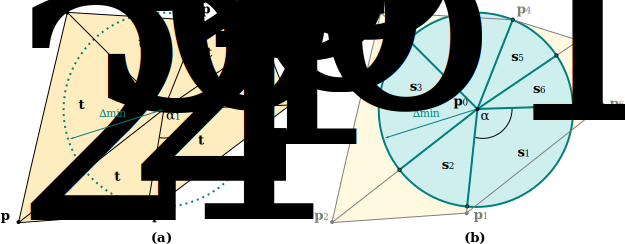
\includegraphics[width=0.5\linewidth]{figures/geodesicDisc.png}}
	{\caption[One-ring and geodesic disc]{A typical one-ring neighborhood $\bN$ with (a) irregular triangular faces $\bt_i$, the smallest edge length $\Dm = |\bp_4 - \bp_0|$ shown here with a teal arrow as the radius of the geodesic disc, and $\alpha_i$ as the central angle of $\bt_i$ (b) the complete geodesic disc $\bG$, comprised of all its circular sectors $\bs_i$, each having central angles $\alpha_i$}\label{fig:geodesicDisc}}
\end{figure}%
\nomenclature[a08]{$\bt_i$}{the triangular faces of $\bN$}%
\nomenclature[a09]{$\bG$}{the geodesic disc about $\bp_0$}%
\nomenclature[a10]{$\bs_i$}{the circle sectors which comprise $\bG$}%
%
\section{Angles}
\label{cFONSsA}
In order to perform the many neccessary trigonometric operations required by the Fast One-Ring smoothing filter, we now compute the inner angles $\alpha_i$ of triangles $\bt_i$ using the using the Law of Cosines. \todoCitation{law of cosines}
\begin{equation}
	\alpha_i = cos^{-1}(\frac{|\bp_0 - \bp_{i}|^2 + |\bp_0 - \bp_{\sipo}|^2 - |\bp_i - \bp_{\sipo}|^2}{2\cdot|\bp_0 - \bp_{i}|\cdot|\bp_0 - \bp_{\sipo}|})
	\label{eq:alphaFromEdgeLengths}
\end{equation}%
\nomenclature[b01]{$\alpha_i$}{the central angle of $\bs_i$}%

We also require For interpolation of the function values over the entire circular sector, we must first interpolate the values one side of the bisecting line at a time. The angles $\beta_i$ are therefore calculated using the third angle theorem as the third angle to form a right triangle along with $\alpha_i\mathbin{/}2$ for each half of $\bs_i$. \todoCitation{and third angle theorems}
\begin{equation}
	\beta_i = \Big(\frac{\pi}{2} - \frac{\alpha_i}{2}\Big) = \frac{(\pi - \alpha_i)}{2}
	\label{eq:betaFromHalfAlpha}
\end{equation}%
\nomenclature[b02]{$\beta_i$}{the third angle with $\frac{\alpha_i}{2}$ and $\frac{\pi}{2}$}%
%
\section{Area \& Center of Gravity}
\label{cFONSsACG}
We also need the area of each circular sector $\bs_i$ comprising the geodesic disc $\bG$ of the one-ring neighborhood $\bN$, which can be calculated with just $\gDm$ and $\alpha_i$
\begin{equation}
	A_i = \frac{(\gDm)^2\alpha_i}{2}
	\label{eq:circularSectorArea}
\end{equation}
\todoCitation{area of circle sectors, http://mathworld.wolfram.com/CircularSector.html}%
\nomenclature[c01]{$A_i$}{area of circular sector $i$}%

Next, the distance from the center point $\bp_0$ to the center of gravity for the circular sector $\bs_i$ is calculated as
\begin{equation}
	\Dc_i := \frac{2\:\gDm\:\sin(\frac{\alpha_i}{2})}{3\:\frac{\alpha_i}{2}}
	\label{eq:distToCoG}
\end{equation}
\todoCitation{area of circle sectors, http://mathworld.wolfram.com/CircularSector.html}%
\nomenclature[c03]{$\Dc_i$}{the distance to $\bc_i$ within $\bs_i$}%

Figure~\ref{fig:centerOfGravity} illustrates the center of gravity, or centroid, \todoCitation{centroid} and its distance from the center point of the circular sector, using $\bs_i$ from Figure~\ref{eq:localMinimumEdgeLength} as an example. In general, the smaller the angle $\alpha_i$ of the circle sector, the longer the distance $\Dc_1$ becomes.
\begin{figure}[ht]
\ffigbox
	{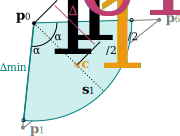
\includegraphics[width=0.6\linewidth]{figures/centerOfGravity.png}}
	{\caption[Distance to and Center of Gravity]{A single circle sector $\bs_1$ with a bisecting line in black dots and its center of gravity $\bc_1$ marked in a sand color, as well as the distance from the center point $\bp_0$ to $\bc_1$ drawn in coral as $\Dc_1$}\label{fig:centerOfGravity}}
\end{figure}%
\nomenclature[c02]{$\bc_i$}{center of gravity (centroid) of $\bs_i$}%
%
\section{Interpolation}
\label{cFONSsI}
With $\alpha_i\mathbin{/}2$, $\beta_i$, and $\gDm$ being constant for both halves of any circular sector $\bs_i$ , we can next use the Law of Sines to obtain a constant ratio by which we can interpolate the three function values at the points $\bp_0$, $\bp_i$, and $\bp_{\sipo}$ which comprise the face $\bt_i$.
\begin{equation}
	\zeta_i = \frac{\gDm}{\sin(\beta_i)}
	\label{eq:zeta}
\end{equation}%
\nomenclature[d01]{$\zeta_i$}{constant ratio for interpolation derived from Law of Sines}%

With the constant ratio $\zeta_i$, we can obtain both of the distances for interpolation. Please note, because the points $\bp_i$ and $\bp_{\sipo}$ are likely at different distances from the center point $\bp_0$, we must now begin calculating for each half of the circular sector individually, therefore we adopt the superscript to denote the index of the sector, as in $\Dz^i$ for $\bs_i$, and the subscipt to denote the side of the sector defined by its point, as in $\Dz_{\sipo}$ is used with $\bp_{\sipo}$.
\begin{align}
	\Dz^i_i & = \kern4pt\frac{\zeta_i}{|\bp_0 - \bp_i|}
	\label{eq:distanceIForInterpolation}\\
	\Dz^i_{\sipo} & = \frac{\zeta_i}{|\bp_0 - \bp_{\sipo}|}
	\label{eq:distanceIp1ForInterpolation}
\end{align}%
\nomenclature[d02]{$\Dz^i_i$}{also $\Dz^i_{\sipo}$, the distances for interpolation of $f_i$ toward $f_0$}%

From the original function values $f_0$, $f_i$, and $f_{\sipo}$, we can now interpolate based on their distances $\Dz^i_i$ and $\Dz^i_{\sipo}$, to become
\begin{align}
	f'_i & = f_0(1 - \Dz^i_i) + f_i\Dz^i_i
	\label{eq:interpolatedFi} \\
	f'_{\sipo} & = f_0(1 - \Dz^i_{\sipo}) + f_{\sipo}\Dz^i_{\sipo}
	\label{eq:interpolatedFip1}
\end{align}%
\nomenclature[d03]{$f'_i$}{also $f'_{\sipo}$, the interpolated values of $f_i$ toward $f_0$}%
%
\section{Weighted Mean}
\label{cFONSsWM}
To calculate the weighted mean function value $f^\bs_i$ at the center of gravity $\bc_i$ of the circle sector $\bs_i$, we must use $f_0$ the function value at $\bp_0$, both interpolated function values $f^{'i}_i$ and $f^{'\sipo}_i$, and the distance to the center of gravity $\Dc_i$, and we obtain
\begin{equation}
	f^\bs_i = f_0(1 - \Dc_i) + \frac{(f^{'i}_i + f^{'\sipo}_i)\Dc_i}{2}
	\label{eq:weightedMeanAtCoGatSector}
\end{equation}%
\nomenclature[e01]{$f^\bs_i$}{the weighted mean function value at $\bc_i$ of $\bs_i$}%

Finally, we can compute the one-ring weighted mean function value at $\bp_0$ by summing all the weighted mean function values from each $\bs_i$ in $\bN$, weighting those again by each sector's area $A_i$, then finally dividing by the total area of the geodesic disc.
\begin{equation}
	\bar{f}_0 := \frac{\sum A_if^{\bs}_i}{\sum A_i} \quad \forall i \in \{1,\ldots,|\bt_v|\}
	\label{eq:meanFuncValAtP0}
\end{equation}%
\nomenclature[e02]{$\bar{f}_0$}{the one-ring weighted mean function value at $\bp_0$}%
\nomenclature[e03]{$|\bt_v|$}{the number of faces $\bt$ in $\bN_v$, always $\geq 2$, typically $\leq 12$}%

The one-ring smoothing filter can be modified to use the median operation, instead of the mean, by using all the equations except ~\ref{eq:meanFuncValAtP0} and then sorting the results of ~\ref{eq:weightedMeanAtCoGatSector}. The details of which can be found by the original publication ~\cite[s.~3.2]{Mara17}, but as it was not implemented in GPGPU for this thesis, we exclude the details here.
%
\section{Summary}
\label{cFONSsS}
In this chapter we presented an updated version of the Fast One-Ring smoothing filter for scalar fields on discrete manifolds, which since its original publication ~\cite[s.~3.2]{Mara17}, now utilizes the entire area of the geodesic disc $A$ for calculating the weighted averages. First, we have illustrated how one can calculate the smallest edge length $\gDm$, interior angles $\alpha$ and $\beta$, the area $A$ of a sector $\bs$ from the geodesic disc, and distance to the centroid (center of gravity) $\Dc$ for any given one-ring neighborhood $\bN$. Next, we provided the equations for interpolating the three function values $f_0$, $f_i$, and $f_{\sipo}$ using the constant ratio $\zeta$ to obtain the weighted mean function value for each $\bs$, and finally the weighted mean function value $\bar{f_0}$ at point ${\bp_0}$ for the entire one-ring neighborhood $\bN$. Convolving this filter with the scalar field of function values at each vertex in a mesh, thus produces a smoothing effect.

In algorithm~\ref{alg:serialPreCalculation}, we precalculate all the edge lengths $\eta$ in $\bM$, and the global minimum edge length $\gDm$.
\begin{algorithm}
	\DontPrintSemicolon
	\SetCommentSty{small}
	\SetKwFor{For}{for}{:}{}

	\SetKwInOut{Input}{Input}\SetKwInOut{Output}{Output}
	\Input{things for filter}
	\Output{new function values}

	\bigskip
	\FuncSty{PreCalculate}\FuncArgSty{(a,b)}\;
\nl	\For{$v\leftarrow 1\;\KwTo\;m$}{
\nl		\For{$k\leftarrow 1\;\KwTo\;n_v$}{
			\linespread{1.5}\selectfont
\nl			$\eta_{vk} \leftarrow |\bp_k - \bp_v|$\tcc*[r]{every edge length}
\nl			$\gDm \leftarrow \min\{\gDm, \eta_{vk}\}$\tcc*[r]{Eq:~\ref{eq:globalMinimumEdgeLength}}
			%TODO:should I include initialization of \gDm to 0?
		}
	}
	\caption{Serial algorithm for the calculations required by the Fast One-Ring smoothing filter, before it can begin its convolution \label{alg:serialPreCalculation}}
\end{algorithm}%
\nomenclature[f01]{$n_i$}{the cardinality of $\bN$ about $\bp_i$}%
\nomenclature[f02]{$\eta_{vk}$}{the length of the edge between $\bp_v$ and $\bp_k$}%

\todoReword{use more and define, or reword convolution in alg:1 caption}
Algorithm~\ref{alg:serialPreCalculation} introduces a few\todoReword{give real number} new symbols: $v$ is used to represent a unique index for each vertex in $\bM$, $k$ indexes each neighbor in the one-ring neighborhood $\bN$ of $\bp_v$, whose cardinality is $n_v$, $|\bp_k-\bp_v|$ from $line3$ is analogous to $|\bp_i-\bp_0|$ from equation~\ref{eq:localMinimumEdgeLength} when $\bp_v$ becomes $\bp_0$, and finally, $\eta_{vk}$ is the length of the edge between $\bp_v$ and $\bp_k$.

In algorithm~\ref{alg:serialCalculate}, we illustrate the remaining steps required to process a mesh using the one-ring filter, after having completed the pre-calculations in~\ref{alg:serialPreCalculation}.
%
\begin{algorithm}
	\DontPrintSemicolon
	\SetCommentSty{small}
	\SetKwFor{For}{for}{:}{}

	\SetKwInOut{Input}{Input}\SetKwInOut{Output}{Output}
	\Input{things for filter}
	\Output{new function values}

	\bigskip
	\linespread{1}\selectfont
	\FuncSty{Calculate}\FuncArgSty{(a,b)}\;
\nl	\For{$v\leftarrow 1\;\KwTo\;m$}{
\nl		\For{$i \leftarrow 1\:\KwTo\:|\bt_v|$}{
			\linespread{1.5}\selectfont
\nl			$\alpha_i \leftarrow \text{cos}^{-1}\big((\eta^v_{0,2})^2 + (\eta^v_{0,1})^2 - (\eta^v_{1,2})^2\big)\mathbin{/}\big(2(\eta^v_{0,2})(\eta^v_{0,1})\big)$\tcc*[r]{Eq:~\ref{eq:alphaFromEdgeLengths}}
\nl			$\beta_i \leftarrow (\pi - \alpha_i)\mathbin{/}2$\tcc*[r]{Eq:~\ref{eq:betaFromHalfAlpha}}
\nl			\kern-2pt$A_i \leftarrow \gDm^2\alpha_i\mathbin{/}2$\tcc*[r]{Eq:~\ref{eq:circularSectorArea}}
\nl			\kern-7pt$\Dc_i \leftarrow \big(2\:\gDm\:\sin(\alpha_i\mathbin{/}2)\big)\mathbin{/}(3\alpha_i\mathbin{/}2)$\tcc*[r]{Eq:~\ref{eq:distToCoG}}
\nl			\kern1pt$\zeta_i \leftarrow \gDm\mathbin{/}\sin(\beta_i)$\tcc*[r]{Eq:~\ref{eq:zeta}}
\nl			\For{$j \in {1,2}$}{
\nl				\kern-8pt$\Dz^i_j \leftarrow \zeta_j\mathbin{/}|\bp_0 - \bp_j|$\tcc*[r]{Eq:~\ref{eq:distanceIForInterpolation},~\ref{eq:distanceIp1ForInterpolation}}
\nl				$f'_j \leftarrow f_0(1 - \Dz^i_j) + f_j\Dz^i_j$\tcc*[r]{Eq:~\ref{eq:meanFuncValAtP0},~\ref{eq:interpolatedFip1}}
			}
\nl			$f^\bs_i \leftarrow f_0(1 - \Dc_i) + \big((f^1_i + f^2_i)\Dc_i\big)\mathbin{/}2$\tcc*[r]{Eq:~\ref{eq:weightedMeanAtCoGatSector}}
\nl			\kern-2pt$\tilde{A}_v \leftarrow \tilde{A}_v + A_i$\tcc*[r]{Eq:~\ref{eq:meanFuncValAtP0}}
\nl			$\tilde{f}_v \leftarrow \tilde{f}_v + A_if^{\bs}_i$\tcc*[r]{Eq:~\ref{eq:meanFuncValAtP0}}
		}

\nl		$\bar{f}_v \leftarrow \tilde{f}_v\mathbin{/}\tilde{A}_v$\tcc*[r]{Eq:~\ref{eq:meanFuncValAtP0}}
	}
	\caption{Serial algorithm for the Fast One-Ring smoothing filter for scalar fields on discrete manifolds\label{alg:serialCalculate}}
\end{algorithm}%
\nomenclature[f03]{$\eta^v_{1,2}$}{the length of the edge between $\bp_i$ and its neighbors in $\bt_i$, $\bp_1$ and $\bp_2$}%


\chapter{Profiling \& Exploiting Concurrency}
\label{ch5}
In the previous chapter we presented an improved version of \Forf{t} as it is currently implemented within the GigaMesh framework, and while it has improved accuracy in regards to the weights, it is still yet entirely serial in design, so that unfortunately, its performance suffers greatly under the complexity of modern mesh sizes, which with the current high resolution scanners in use, can grow to be MESH\_SIZES\todoResearch{mesh sizes}. We will now explore this as-yet-unpublished algorithm in order to negotiate any instances of control or data dependency, and hopefully discover opportunities worthy of exploiting concurrency in order to improve its performance when implemented on a system capable of parallel computation.

%
%
%
%
\section{The Serial Algorithm}
\label{ch5sSI}
In this section, we now combine all of the equations from the previous chapter,~\ref{eq:localMinimumEdgeLength} through~\ref{eq:meanFuncValAtPv}, into a three-part algorithm using mathematical pseudo-code, with the goal of facilitating the implementation of the improved version of \forf{t}. To that end, before one is able to actually begin convolving the filter, the computations require that the one-ring neighborhoods already be known. Also, during the convolutions, the filter uses all edge lengths at least once per iteration, and twice for non-border edge lengths, which are shared between adjacent neighborhoods. Therefore, it is beneficial to split the algorithm into three distinct parts, then save the results of the first two parts to be used during the iterative convolutions of the third part, with the result being a massive increase in efficiency by greatly reducing the number of operations-per-iteration required.
\todoBackground{add convolution and convolve to background}
\todoBackground{memory vs speed cost compromise}

%
%
\subsection{Discovering Neighborhoods}
\label{ch5sSIssDN}
Initially, one must discover all the points $\bp_i$ which comprise each neighborhood $\bN_v$ in the entire mesh $\bM$, which is the purpose of Algorithm~\ref{alg:serialBuildNeighborhoods}. Although building this family of sets outside of the principle loop adds an additional $2\cdot |\bT|^3$ operations in total, doing so enables Alogrithm~\ref{alg:serialCalculateEdgeLengths} to exploit this family of sets to vastly reduce its complexity from $|\bP|^{|\bT|}$ to approximately\footnote{depending on the average size of all neighborhoods, assumed here to be about 6}\todoResearch{find good average for average neighborhood size} $|\bP|^6$. Also, as we will see in Algorithm~\ref{alg:serialConvolveFilter}, when $\tau$ is the chosen number of iterations to perform, the complexity of the main procedure can be meaningfully reduced to only $\tau^{|\bP|^{6*3}}$, down from the $\tau^{|\bP|^{(|\bF|*3)}}$ that would have been necessary had the neighborhoods not already been discovered and the procedure been otherwise required to discover the members of $\bN_v$ in each iteration.%
\nomenclature[na]{$\tau$}{the chosen number of iterations to perform}%
\todoBackground{complexity, big O notation}

Figure~\ref{fig:serialBuildNeighborhoods} describes a very simple mesh consisting of just four points and two faces, similar to what is seen in Figure~\ref{fig:triangularFaces}. The two faces, $\bt_1$ and $\bt_2$, are colored in sand and coral color respectively. The arrows represent the union operation of a point and a neighborhood, and are colored to match the face from where the point had come. The two pairs of arrows pointing from $\bp_2$ to $\bN_3$ and $\bp_3$ to $\bN_2$ are specifically colored teal to highlight the fact that these union operations occur twice, originating one each from each of the faces, but because of the uniqueness property of a set, the duplicated operations are wholly inconsequential to the the final membership of either neighborhood. Also notice that for every face which contains its center point, the union operation is called twice on neighborhood. This realization will eventually influence the design of the parallel variant of the algorithm.

\tikzset{%
	>={Latex[width=2mm,length=2mm]},
	baseNode/.style = {rectangle, rounded corners,
		draw=black, fill=white, thick,
		minimum width=1cm, minimum height=1cm,
		text centered, font=\sffamily},
	baseLine/.style = {double, thick},
	tealStyle/.style = {draw=MyTeal, fill=MyLtTeal},
	coralStyle/.style = {draw=MyCoral, fill=MyLtCoral},
	sandStyle/.style = {draw=MySand, fill=MyLtSand},
	faceL/.style = {baseNode, sandStyle},
	lineL/.style = {baseLine, sandStyle},
	faceR/.style = {baseNode, coralStyle},
	lineR/.style = {baseLine, coralStyle},
	lineC/.style = {baseLine, tealStyle},
	point/.style = {baseNode},
	nbhd/.style = {baseNode, minimum width=2cm}
}
\begin{figure}[ht]
	\begin{tikzpicture}[node distance=0cm]
		\coordinate (center1) at (0cm,0cm);
		\node (t1) [faceL, anchor=east, xshift=-.5cm] {$\bt_1 = \{\bp_1,\,\bp_2,\,\bp_3\}$};
		\node (t2) [faceR, anchor=west, xshift= .5cm] {$\bt_2 = \{\bp_3,\,\bp_2,\,\bp_4\}$};
		\coordinate (center2) at (0cm,-1.5cm);
		\node (p1) [point, left of=center2, xshift=-3cm] {$\bp_1$};
		\node (p2) [point, left of=center2, xshift=-1cm] {$\bp_2$};
		\node (p3) [point, right of=center2, xshift=1cm] {$\bp_3$};
		\node (p4) [point, right of=center2, xshift=3cm] {$\bp_4$};
		\coordinate (center3) at (0cm,-4.5cm);
		\node (n1) [nbhd, left of=center3, xshift=-5cm] {$\bN_1$};
		\node (n2) [nbhd, left of=center3, xshift=-1.75cm] {$\bN_2$};
		\node (n3) [nbhd, right of=center3, xshift=1.75cm] {$\bN_3$};
		\node (n4) [nbhd, right of=center3, xshift=5cm] {$\bN_4$};

		\draw[-, lineL] (t1) -- (p1);
		\draw[-, lineL] (t1) -- (p2);
		\draw[-, lineL] (t1) -- (p3);

		\draw[->, lineL] (p1) -- (n2);
		\draw[->, lineL] (p1) -- (n3);
		\draw[->, lineL] (p2) -- (n1);
		\draw[->, lineC] (p2) -- (n3.180);
		\draw[->, lineL] (p3) -- (n1);
		\draw[->, lineC] (p3) -- (n2);

		\draw[-, lineR] (t2) -- (p2);
		\draw[-, lineR] (t2) -- (p3);
		\draw[-, lineR] (t2) -- (p4);

		\draw[->, lineC] (p3) -- (n2.0);
		\draw[->, lineR] (p3) -- (n4);
		\draw[->, lineR] (p2) -- (n4);
		\draw[->, lineC] (p2) -- (n3);
		\draw[->, lineR] (p4) -- (n3);
		\draw[->, lineR] (p4) -- (n2);
	\end{tikzpicture}
	{\caption[Serial Build Neighborhoods]{A very simple mesh consisting of just four points and two faces, similar to what is seen in Figure~\ref{fig:triangularFaces}. $\bt_1$ is in sand color, and $\bt_2$ is in coral color. The arrows represent the union operation of a point into a neighborhood, and are colored to match the face from where the point had come. The two pairs of arrows pointing from $\bp_2$ to $\bN_3$ and $\bp_3$ to $\bN_2$ are colored in teal to highlight the fact that these union operations occur twice.
}\label{fig:serialBuildNeighborhoods}}
\end{figure}

In Algorithm~\ref{alg:serialBuildNeighborhoods}, the function \textit{serialBuildNeighborhoods} describes iterating over every triangular face $\bt$ in $\bT$, then for each of the face's three corner points, union into its neighborhood the other two points which are adjacent to it. The result is a fully populated family of sets $\bN$, storing references to every neighbor of every neighborhood in the mesh.

\begin{algorithm}[ht]
	\DontPrintSemicolon
	\SetCommentSty{small}
	\SetKwFor{For}{for}{:}{}
	\SetKwProg{Func}{Function}{}{}
	\SetKwInOut{Input}{Input}\SetKwInOut{Output}{Output}

	\Input{the set of all triangular faces $\bT$}
	\Output{the family of sets of discovered neighborhoods $\bN$}

	\bigskip
\nl	\Func{serialBuildNeighborhoods($\bT$)}{\label{sbn1}
\nl		\For(\tcc*[f]{$\bt = \left \{\bp_a, \bp_b, \bp_c\right \}$}){$\bt \in \bT$}{\label{sbn2}
\nl			\ProgSty{union($\bN$, $\bp_a$, $\bp_b$, $\bp_c$)}\;\label{sbn3}
\nl			\ProgSty{union($\bN$, $\bp_b$, $\bp_a$, $\bp_c$)}\;\label{sbn4}
\nl			\ProgSty{union($\bN$, $\bp_c$, $\bp_a$, $\bp_b$)}\;\label{sbn5}
		}
	}

	\bigskip
\nl	\Func{union($\bN$, $a$, $b$, $c$)}{\label{sbn7}
\nl		$\bN_a \leftarrow \bN_a \cup \{b,\,c\}$\;\label{sbn8}
	}
	\caption{Serial algorithm for building the family of sets of all discovered members of each neighborhood in the mesh\label{alg:serialBuildNeighborhoods}}
\end{algorithm}%

The function ``union'' is separated here for two reasons: the first reason is that this way, it becomes very clear that the union operation behaves similarly for all three permutations\footnote{In general, a set of three numbers has six permutations, however, here only the first index is important, and the order of the second two parameters are arbitrary due to the commutative property of the union operation, resulting in only 3 distinct possibilities} of corners, and indeed it is only the order of the indices which changes; and the second reason is that this signature matches more closely that of the parallel version, Algorithm~\ref{alg:parallelBuildNeighborhoods}, which requires the union operation to remain separate.
\todoBackground{Commutative property of union operation}

%
%
\subsection{Calculating Edge Lengths}
\label{ch5sSIssCEL}
Having now built in the previous section the family of sets of neighborhoods $\bN$, we can advance to the next step, Algorithm~\ref{alg:parallelCalculateEdgeLengths}, which iterates over each pair of neighbors comprising $\bN$, with the goal of building a set of pre-calculated edge lengths $\bE$, as well as determining the global minimum edge length $\gelm$; both being essential parameters of Algorithm~\ref{alg:serialConvolveFilter}.

As shown in Equation~\ref{eq:defineEdgeLengthPoint}, the calculation of an edge's length requires taking the L2-norm of the difference between two points, which itself involves using the square root operation. In modern software, the square root operation is performed by computing ``Newton's Iteration'', or ``Newton's method''\todoCitation{software uses Newton's iteration for sqrt}, which is essentially multiple iterations of the so-called, ``recurrence equation''.~\cite{Weisstein19b}\todoCitation{Newton's iteration uses recurrence equation} The impact for \forf{t} is that the computation of a square root typically\todoReword{add footnote with desc and citation}\todoCitation{how slow is Newton's iteration compared to others} takes many more compute cycles than  any other binary or unary operation, thus taking more time to complete overall. In fact, because of the slowness of the square root operation, computing the L2-norm in order to calculate an edge's length is empirically the most costly operation performed by the filter\todoResearch{qualify, do experiment to prove how slow sqrt is, maybe make appendix entry about what it is and why it is so slow}. Therefore, it is imperative that we pay special attention to avoid unnecessary instructions to calculate an edge's length. For that reason, we define the symbol $\ellstar$ to represent the calculation of an edge's length using ``Newton's Iteration'', so as to draw focus to its importance while designing an efficient implementation of \forf{t}.%
\nomenclature[oa]{$\ellstar$}{the procedure of calculating an edge's length using ``Newton's Iteration'', the most costly operation in the Fast One-Ring filter, due to use of $\sqrt{(\cdot)}$}

\begin{algorithm}[ht]
	\DontPrintSemicolon
	\SetCommentSty{small}
	\SetKwFor{For}{for}{:}{}
	\SetKwProg{Func}{Function}{}{}
	\SetKwInOut{Input}{Input}\SetKwInOut{Output}{Output}

	\Input{the set of all points $\bP$, \\
		the family of sets of discovered neighborhoods $\bN$}
	\Output{the set of pre-calculated edge lengths $\bE$, \\
		the globally shortest edge length $\gelm$}

	\bigskip
	\Func{serialCalculateEdgeLengths($\bP$, $\bN$)}{
\nl		\For{$\bp_v \in \bP$}{\label{scel1}
\nl			\For{$\bp_i \in \bN_v$}{\label{scel2}
				\linespread{1.5}\selectfont
\nl				$\bE_{\sv{i}} \leftarrow |\bp_i - \bp_v|$\tcc*[r]{This is $\ellstar$ as in Eq:~\ref{eq:localMinimumEdgeLength}}\label{scel3}
\nl				$\gelm \leftarrow \min\left \{\gelm,\,\ell_{\sv{i}}\right \}$\tcc*[r]{Eq:~\ref{eq:globalMinimumEdgeLength}}\label{scel5}
			}
		}
	}
	\caption{Serial algorithm for calculating all the edge lengths between each pair of adjacent points in the mesh\label{alg:serialCalculateEdgeLengths}}
\end{algorithm}

Given the substantial impact of computing ${\ellstar}$ and the enormous number of times\todoReword{how many times} an edge length is required in the computation of the weighted mean function values per iteration of the filter on a mesh, pre-calculating the set all edge lengths outside of the principle loop becomes critical to the overall efficiency of the algorithm, despite the fact that it requires ${\ellstar}$ to be calculated and stored about $|\bP|^6$ times\footnote{depending on the average size of all neighborhoods, but assumed here to be about 6.}. It is of paramount importance for two reasons: the first reason is that without pre-calcuating each edge length, it would be otherwise impossible to calculate the global minimum  edge length $\gelm$, which is used in every iteration of the principle loop; and the second reason is that by recording the results of each edge length calculation in the set $\bE$, we are then able to completely exclude any further calculations of $\ellstar$ from the principle loop, and as can be seen in Algorithm~\ref{alg:serialConvolveFilter}, that reduces the total count of $\ellstar$ calculations performed by the filter down from the $(2\,\ell_{\sv{i}}^{\,border} + 4\,\ell_{\sv{i}}^{\,non-border})\cdot\tau^{|\bP|}$ had the procedure been required to calculate an edge length each time it was used during computation, to only the initial $1\cdot |\bP|^6$ pre-calculations; having become completely independent of $\tau$ and significantly more efficient overall.%
\nomenclature[ob]{$\bE$}{a set of pre-calculated edge lengths}%
\todoBackground{memory vs speed cost compromise}
\todoBackground{border vs non-border edge lengths}
\todoReword{three big paragraphs in a row is not pretty}

%
%
\subsection{Convolving the Filter}
\label{ch5sSIssCF}
In the third and final part, we present Algorithm~\ref{alg:serialConvolveFilter}, which describes the remaining steps required to convolve \Forf{t}. After having completed the discovery and pre-calculations of Algorithms~\ref{alg:serialBuildNeighborhoods} and~\ref{alg:serialCalculateEdgeLengths}, each convolution is performed for a user-defined number of iterations $\tau$, by convolving over each point $\bp_v$ in the set $\bP$. At each point, the neighboring points $\bp_i$ from set $\bN_v$ are then iterated over, in order to calculate each weighted mean function value $\check{f}$ at the center of gravity of the circle sector defined by $\bp_v$ and $\bp_i$. Next, the weighted mean $f'_v$ is evaluated with all the mean function values from the circle sectors comprising the geodesic disc centered on $\bp_v$,  and is then recorded in set $\bF'$, before \forf{t} finally moves to the next point in the mesh and its corresponding one-ring neighborhood.

\begin{algorithm}[ht]
	\DontPrintSemicolon
	\SetCommentSty{small}
	\SetKwFor{For}{for}{:}{}
	\SetKwProg{Func}{Function}{}{}
	\SetKwInOut{Input}{Input}\SetKwInOut{Output}{Output}

	\Input{the set of all points $\bP$, \\
		the family of sets of discovered neighborhoods $\bN$, \\
		the set of pre-calculated edge lengths $\bE$, \\
		the globally shortest edge length $\gelm$, \\
		the set of function values $\bF$, \\
		the chosen number of iterations $\tau$}
	\Output{the set of one-ring weighted mean function values $\bF'$}

	\bigskip
	\linespread{1}\selectfont
	\Func{convolveFilter($\bP$, $\bN$, $\bE$, $\gelm$, $\bF$, $\tau$)}{
\nl		\For{$\tau\leftarrow 1\;\KwTo\;\#iterations$}{
\nl			\For{$\bp_v \in \bP$}{
\nl				\For{$\bp_i \in \bN_v$}{
					\linespread{1.5}\selectfont
\nl					$\kern-0.5pt\alpha \leftarrow cos^{-1}$
					\begin{Large}
						$\kern-6pt\left (\frac{\bE_c^2\,+\,\bE_b^2\,-\,\bE_a^2}{2\,\cdot\,\bE_c\,\cdot\,\bE_b}\right )$\tcc*[r]{Eq:~\ref{eq:alphaFromEdgeLengths}}
					\end{Large}
					\linespread{1.2}\selectfont
\nl					$\kern0.00pt\beta \leftarrow (\pi - \alpha)\mathbin{/}2$\tcc*[r]{Eq:~\ref{eq:betaFromHalfAlpha}}
\nl					$\kern-1.5ptA \leftarrow \Big(\gelm\,\Big)^2\kern-4pt\cdot\alpha\mathbin{/}2$\tcc*[r]{Eq:~\ref{eq:circularSectorArea}}
\nl					$\kern1.00pt\check{\ell} \leftarrow \big(4\cdot\gelm\cdot\sin(\alpha\mathbin{/}2)\big)\mathbin{/}3\,\alpha$\tcc*[r]{Eq:~\ref{eq:distToCoG}}
\nl					$\kern1.00pt\zeta \leftarrow \gelm\mathbin{/}\sin(\beta)$\tcc*[r]{Eq:~\ref{eq:zeta}}
\nl					\For{$j \in {1,2}$}{
\nl						$\tilde{\ell}_j \leftarrow \zeta\mathbin{/}\bE_j$\tcc*[r]{Eq:~\ref{eq:distanceIForInterpolation},~\ref{eq:distanceIp1ForInterpolation}}
\nl						$f'_j \leftarrow f_0\cdot(1 - \tilde{\ell}_j) + f_j\cdot\tilde{\ell}_j$\tcc*[r]{Eq:~\ref{eq:interpolatedFi},~\ref{eq:interpolatedFip1}}
					}
\nl					$\check{f} \leftarrow f_0\cdot(1 - \check{\ell}) + \big((f'_1 + f'_2)\cdot\check{\ell}\big)\mathbin{/}2$\tcc*[r]{Eq:~\ref{eq:weightedMeanAtCoGatSector}}
\nl					$\kern-2.0pt\tilde{f}_v \leftarrow \tilde{f}_v + A\cdot\check{f}$\tcc*[r]{Eq:~\ref{eq:meanFuncValAtPv}}
\nl					$\kern-4.0pt\tilde{A}_v \leftarrow \tilde{A}_v + A$\tcc*[r]{Eq:~\ref{eq:meanFuncValAtPv}}
				}
\nl				$f'_v \leftarrow \tilde{f}_v\mathbin{/}\tilde{A}_v$\tcc*[r]{Eq:~\ref{eq:meanFuncValAtPv}}
			}
		}
\nl		$\bF' \leftarrow \left \{f'_1,\ldots,\,f'_{|\bP|}\right \}$\;
\nl 	$\bF \leftarrow \bF'$\tcc*{smooth newest values every iteration}
	}
	\caption{Serial algorithm for convolving \Forf{t}\label{alg:serialConvolveFilter}}
\end{algorithm}%
\nomenclature[pa]{$\tilde{f}$}{the total volume of function values over $\bO_v$}%
\nomenclature[pb]{$\tilde{A}$}{the area of $\bO_v$}%
\nomenclature[]{$\bF'$}{the set of one-ring weighted mean function values}%

While the performance of Algorithm~\ref{alg:serialConvolveFilter} is much improved with the pre-calculations performed in Algorithms~\ref{alg:serialBuildNeighborhoods} and~\ref{alg:serialCalculateEdgeLengths}, its strictly serial design prevents it from scaling in performance appropriately for the sizes of real-world, acquired \tdd{}, performing especially sluggishly for high numbers of iterations on meshes with large amounts of triangulated points\todoReference{a specific experiment} the very targets for which the filter is primarily intended.

In this section, we presented an improved version of \Forf{t}, as implemented within the GigaMesh framework. Unfortunately, it is still yet entirely serial in design, therefore, we will in the next section, endeavor to explore this as-yet-unpublished algorithm in order to discover possible occurrences of independent procedures worthy of exploiting with parallel processing, with the goal of improving the overall performance and scalability of \forf{t} when it is implemented on a system capable of parallel computation.


%
%
%
%
\section{The Parallel Algorithm}
\label{ch5sPA}
\todoBackground{Data dependencies}
Following the pattern set in Section~\ref{ch5sSI}, the parallel algorithm for \Forf{t} also has three main parts. In contrast however, the parallel variant of each of the three serial parts are split further into subroutines, in order to delegate blocks of instructions to separate threads of execution, while protecting critical sections, and avoiding data and control dependencies, so that the threads can be safely executed in parallel.

The following three sections will each focus on producing the parallel variant of one of the three parts of the serial algorithm, by first analyzing the serial algorithm through the lens of parallel programing, then defining the strategy behind the design of the parallel variant, then finally providing the pseudo code definitions to implement that part of the algorithm.

%
%
\subsection{Discovering Neighborhoods}
\label{ch5sPAssDN}
The sole purpose of Algorithm~\ref{alg:serialBuildNeighborhoods} is to generate a family of sets of neighborhoods $\bN$, by exploring every triangular face in the set, so that subsequent algorithms can recall and iterate over those associations without incurring the computational cost of searching the entire mesh each time. In addition to that goal, the parallel variant of the $\mathit{buildNeighborhoods}$ procedure should also provide a total count of all neighbors in all neighborhoods $\hat{n}$, so that the next two parts of the \forf{t} algorithm can predict and evenly delegate work loads to independent threads of execution.

In Algorithm~\ref{alg:serialBuildNeighborhoods}, line~\ref{sbn2}, the first line of the first function, we encounter a loop over each face $\bt$ in $\bT$. In general, concurrency found in the structure of a loop may be totally exploited by parallel systems, but only in the absence of loop-carried dependence. So, in order to determine if the iterations of the loop may be computed in parallel, an analysis of every operation in the loop block is required.\todoResearch{Amdahl's Law}\todoBackground{loop level parallelism, loop-carried and loop-independent}
\todoBackground{static vs volatile memory}

Figure~\ref{fig:paraBNDataDep} illustrates the data dependencies inherent to each iteration of the loop over the faces $\bt$ in $\bT$, as found from Algorithm~\ref{alg:serialBuildNeighborhoods}. First the triangular face $\bt$ is loaded, as denoted by the teal colored node, from the set $\bT$ in static memory which will never be modified by this, or any other procedure. Also, despite the fact that faces can be adjacent to one another, each face is distinctly defined in the set $\bT$, therefore, each face $\bt$ can be considered independent of each other face. Thus, this first instruction of the loop block is free from any control or data dependencies. The next line in the algorithm is a complex instruction, though, so it must be analyzed in parts.

The first part of the instruction on line~\ref{sbn3}, as denoted by the first three teal colored lines, is to read from face $\bt$ stored in static memory, the indices of the three points $\bp_a$, $\bp_b$, $\bp_c$. Because the face $\bt$ is independent, reading the indices of its three points is also free of dependencies. Next, $\bp_a$ is referenced in order to read the state of $\bN_a$ from volatile memory, as denoted as teal and coral colored lines, respectively. $\bN_a$ is stored in volatile memory, which may potentially be modified by other threads, because it is not known a priori which thread will discover the points which belong to that neighborhood, thus it must be accessible to any and all threads. Next, drawn in sand color, are the two union operations performed in succession on $\bN_a$ with the points $\bp_b$, then $\bp_c$. While these two operations are themselves independent, being performed only on values currently immutable by other procedures, they do rely on having already read the status of $\bN_a$, which indeed does have its own data dependence, hence the sand coloring. Finally illustrated as a double, coral colored arrow, the  the updated set $\bN_a$ is saved back into $\bN$ in volatile memory.

\tikzset{%
	>={Latex[width=2mm,length=2mm]},
	baseNode/.style = {rectangle, rounded corners,
		draw=black, fill=white, thick,
		minimum width=1cm, minimum height=1cm,
		text centered, font=\sffamily, inner sep=.2cm},
	baseLine/.style = {thick},%double},
	tealStyle/.style = {draw=MyTeal, fill=MyLtTeal},
	coralStyle/.style = {draw=MyCoral, fill=MyLtCoral},
	sandStyle/.style = {draw=MySand, fill=MyLtSand},
	%
	indNode/.style = {baseNode, tealStyle},
	indLine/.style = {baseLine, draw=MyTeal},
	depNode/.style = {baseNode, coralStyle},
	depLine/.style = {baseLine, draw=MyCoral},
	mixNode/.style = {baseNode, sandStyle},
	mixLine/.style = {baseLine, draw=MySand},
}
\begin{figure}[ht]
	\begin{tikzpicture}[node distance=0cm]
		\coordinate (center1) at (0cm,0cm);
		\node (sm) [indNode, xshift=-2.25cm] {$\bt$ in static memory};
		\node (vm) [depNode, anchor=west, xshift= 1.25cm] {$\bN$ in volatile memory};

		\coordinate (center2) at (0cm,-2cm);
		\node (pc) [indNode, left of=center2, xshift=-3.50cm] {$\bp_c$};
		\node (pb) [indNode, left of=center2, xshift=-2.25cm] {$\bp_b$};
		\node (pa) [indNode, left of=center2, xshift=-1.00cm] {$\bp_a$};

		\node (Na) [depNode, right of=center2, xshift=1.00cm, yshift=-.5cm] {$\bN_a$};

		\node (union1) at (0cm,-4cm) [mixNode] {$\bN_a \cup \{\bp_b\}$};

		\node (union2) at (0cm,-5.5cm) [mixNode] {$\bN_a \cup \{\bp_c\}$};

		%
		\draw[->, indLine] (sm) -- (pa);
		\draw[->, indLine] (sm) -- (pb);
		\draw[->, indLine] (sm) -- (pc);
		\draw[->, depLine] (vm.220) -- (Na);
		\draw[->, indLine] (pa.east) -- (Na.west);

		\draw[->, indLine] (pb.south) .. controls (-1.75cm,-3.5cm) .. (union1.west);
		\draw[->, mixLine] (Na) -- (union1.north);

		\draw[->, indLine] (pc.south) .. controls (-2cm,-5cm) .. (union2.west);
		\draw[->, mixLine] (union1) -- (union2);
		\draw[->, depLine, double] (union2.east) .. controls (2cm,-5cm) .. (vm);

	\end{tikzpicture}
	{\caption[Data Dependencies in Algorithm for Parallel Build Neighborhoods]{illustrates the data dependencies as found in Algorithm~\ref{alg:serialBuildNeighborhoods}. Operations with data dependencies are in coral color, independent operations are in teal color, and independent operations which reply on operations which have dependencies are in sand color.}\label{fig:paraBNDataDep}}
\end{figure}

Both reading from, and writing to $\bN_a$ in volatile memory constitutes a critical section in the algorithm, which must be accounted for in the design of the parallel variant. Furthermore, both dependencies lie in a single path of dependence, which means that the entire group of operations must be protected by a guarding mechanism as described in Section~\ref{ch2sPPssMS}. Fortunately, because both dependencies revolve around the same set $\bN_a$, a simple mutex per neighborhood will be sufficient. Lines~\ref{sbn4} and~\ref{sbn5} behave similarly to line~\ref{sbn3}, except they concern other neighborhoods, which in turn, need their own mutexes.\todoBackground{path of dependence} Fortunately, by exploiting the fact that the union operation is called exactly twice per each neighborhood for every face which contains its center point, by executing these two operations sequentially within a single mutex, one can mitigate exactly half of the possible collisions in the $\mathit{buildNeighborhoods}$ procedure.

Algorithm~\ref{alg:parallelBuildNeighborhoods} defines the structure and instructions required to implement a parallel variant of the serial procedure, $\mathit{buildNeighborhoods}$, and ensuring correctness by using a set of mutexes. The main function requires only the number of available processors $\rho$, the set of all triangular faces $\bT$, and the cardinality of the set of points $|\bP|$. First, the stride is calculated as the problem size with the unit of work being a single face $\bt$, divided by the number of available processors. Next, a set of mutexes is defined, containing the $|\bP|$ amount of mutexes to be used one each for each neighborhood. \todoReword{remove if no longer setting $\bM$} Then begins the loop to spawn a ``build'' thread for a quarter of the available processors in the system, with the scalar 4 being a result of each build thread's need to spawn 3 additional ``union'' threads. Finally, all the working threads must first synchronize before the family of sets $\bN$ can be realized.

Along with access to the set of triangular face $\bT|$ and set of mutexes $\bM$, each build thread in Algorithm~\ref{alg:parallelBuildNeighborhoods} also requires an index $\Pi$, which it uses along with the stride size $sigma$, to calculate the lower and upper boundaries, $\check{\sigma}$ and $\hat{\sigma}$, for the stride of the problem on which it should compute. Next, it iterates over each face $\bt$ within those stride boundaries, and spawns three union threads; one each for the three points comprising the corners of the current triangular face. Each union thread requires access to not only the family of sets of neighborhoods $\bN$ and the set of mutexes $\bM$, but also the index of the point which it will consider to be central, and two indices of the points which are neighboring it. With those inputs, each union thread then attempts to lock the mutex with the matching index of the central point, blocking until it is able to do so, in order to safely perform the union operation with the currently known neighborhood of the central point, and the set of its two newly discovered neighbors; finally, saving the updated neighborhood to shared memory, then unlocking the mutex.

\begin{algorithm}[ht]
	\DontPrintSemicolon
	\SetCommentSty{small}
	\SetKwFor{For}{for}{:}{}
	\SetKwProg{Func}{Function}{}{}
	\SetKwInOut{Input}{Input}\SetKwInOut{Output}{Output}

	\Input{the number of available processors $\rho$, \\
		the set of all triangular faces $\bT$, \\
		the cardinality of the set of points $|\bP|$}
	\Output{the family of sets of discovered neighborhoods $\bN$}

	\bigskip
\nl	\Func{parallelBuildNeighborhoods($\rho$, $\bT$, $|\bP|$)}{
\nl		$\sigma \leftarrow |\bT|\mathbin{/}\rho$\tcc*{assuming an integer quotient}
\nl		$\fM \leftarrow \{\mu_1,\,\ldots,\,\mu_{|\bP|}\}$\;
\nl		\For{$\Pi \leftarrow 1$ \KwTo $\rho\mathbin{/}4$}{
\nl			\ProgSty{$\sim$build($\Pi$, $\sigma$, $\fM$, $\bT$)}\;
		}

		\medskip
\nl		\ProgSty{synchronizeThreads()}\;
		\medskip
	}

	\bigskip
\nl	\Func{build($\Pi$, $\sigma$, $\fM$, $\bT$)}{
\nl		$\check{\sigma} \leftarrow (\Pi-1)\,\sigma+1$\tcc*{works through its stride}
\nl		$\hat{\sigma} \leftarrow \Pi\,\sigma$\;
\nl		\For(\tcc*[f]{$\bt = \left \{\bp_a, \bp_b, \bp_c\right \}$}){$\bt \in \{\bt_{\check{\sigma}},\ldots,\,\bt_{\hat{\sigma}}\}$}{
\nl			\ProgSty{$\sim$safeUnion($\fM$, $\bN$, $\bp_a$, $\bp_b$, $\bp_c$)}\;
\nl			\ProgSty{$\sim$safeUnion($\fM$, $\bN$, $\bp_b$, $\bp_a$, $\bp_c$)}\;
\nl			\ProgSty{$\sim$safeUnion($\fM$, $\bN$, $\bp_c$, $\bp_a$, $\bp_b$)}\;
		}
	}

	\bigskip
\nl	\Func{safeUnion($\fM$, $\bN$, $a$, $b$, $c$)}{
\nl		$\ProcSty{lock}(\mu_a)$\;
\nl		$\bN_a \leftarrow \bN_a \cup \{b,\,c\}$\;
\nl		$\ProcSty{unlock}(\mu_a)$\;
	}
	\caption{Parallel algorithm for building the family of sets of all members of each neighborhood discovered in the mesh \label{alg:parallelBuildNeighborhoods}}
\end{algorithm}%
\nomenclature[]{$\rho$}{the number of available processors}%
\nomenclature[]{$\sigma$}{the ``stride'', the size of a block of work intended for a single processor, equal to the problem size divided by the number of available processors}%
\nomenclature[]{$\check{\sigma}$}{the index of the beginning of a stride}%
\nomenclature[]{$\hat{\sigma}$}{the index of the beginning of a stride}%
\nomenclature[]{$\Pi$}{a process, to be executed}%
\nomenclature[]{$\fM$}{a set of mutexes}%
\nomenclature[]{$\mu_v$}{a specific mutex}%
\nomenclature[]{$\sim process()$}{a process to be run in a new thread}%
\todoAsk{use KwTo or \{...\}?}
\todoAsk{remove the "main" function in each algorithm (except the 5)?}
\todoAsk{define $\bM$, set it as an input, or just use it?}

The motivation for Algorithm~\ref{alg:parallelRecursiveCensusNeighborhoods} is that a total count of all neighbors in all neighborhoods $\hat{n}$, should be provided so that the work load incurred by loops found in the next two parts of \forf{t} algorithm, which iterate over each neighbor in the family of sets $\bN$, can be predicted and evenly delegated to each independent thread of execution. While a running sum of cardinalities could be implemented within Algorithm~\ref{alg:parallelBuildNeighborhoods}, unlike in the serial version, it would very inefficient due to the added overhead of collisions with the guarding mechanism required to protect the total sum.  Algorithm~\ref{alg:parallelRecursiveCensusNeighborhoods} only requires as inputs a pre-built family of sets of neighborhoods $\bN$, and the number of processors available in the system, but is highly parallel and performs at a rate of $O(log_2(n))$,\todoReword{not sure how to word bigOrate} so when using a system with multiple processors, it is a much or efficient alternative to calculating the sum implicitly while building $\bN$.

As Algorithm~\ref{alg:parallelRecursiveCensusNeighborhoods} is a recursive algorithm, it can be described by splitting it into three distinct parts. The first part, ``the termination clause'', is defined as when the cardinality of the current subset of $\bN$ is only two, evaluate the sum of each member $\bN_i$, then return the sum of all the results. Not that this ignores the trivial edge case of families of sets with a very small cardinality of less than three. In all other cases, when the cardinality of the current subset of $\bN$ is greater than two, the second part, ``working towards the termination state'', begins. The second part of this recursive strategy describes summing in parallel, the cardinality or value of each adjacent pair of members in the current subset of $\bN$, then saving the sum of each addition in a new ordered subset of integers $\widetilde{\bN}$, which will have half the cardinality of the current subset. In the third and final part, ``the recursive call'', the function \textit{parallelRecursiveCensusNeighborhoods} calls itself using the new subset $\widetilde{\bN}$ as a parameter instead of the original $\bN$.
\todoReword{big O remark at end is too sudden}
\todoBackground{recursive algorithms, three parts}

\begin{algorithm}[ht]
	\DontPrintSemicolon
	\SetCommentSty{small}
	\SetKwFor{For}{for}{:}{}
	\SetKwProg{Func}{Function}{}{}
	\SetKwInOut{Input}{Input}\SetKwInOut{Output}{Output}

	\Input{the number of available processors $\rho$, \\
		the family of sets of neighborhoods $\bN$}
	\Output{the count of all neighbors in all neighborhoods $\hat{n}$}

	\bigskip
\nl	\Func{parallelRecursiveCensusNeighborhoods($\rho$, $\bN$)}{
\nl		\eIf{$|\bN| \leq 2$}{
\nl			$\hat{n} \leftarrow \sum_{i=1}^{|\bN|}\bN_i$\;%\underset{i=1}{\overset{|\bN|}{\sum}}|\bN_i|$\;
		}{%Else
\nl			$\sigma \leftarrow |\bN|\mathbin{/}(2\,\rho)$\;
\nl			\For{$\Pi \in \{1,\ldots,\rho\}$}{
\nl				\ProgSty{$\sim$parallelSum($\Pi$, $\sigma$, $\bN$)}\;
			}
			\medskip
\nl			\ProgSty{synchronizeThreads()}\;
			\medskip
\nl			\ProgSty{parallelRecursiveCensusNeighborhoods($\rho$, $\widetilde{\bN}$)}\;
		}
	}

	\bigskip
\nl	\Func{parallelSum($\Pi$, $\sigma$, $\bN$)}{
\nl		$\check{\sigma} \leftarrow (\Pi-1)\,\sigma+1$\;
\nl		$\hat{\sigma} \leftarrow 2\,\Pi\,\sigma$\;
\nl		\For{$v \in \{\check{\sigma},\,\check{\sigma}\sps{}2,\,\check{\sigma}\sps{}4,\ldots,\,\hat{\sigma}\}$}{
\nl			\eIf(\tcc*[f]{only occurs in first call}){$\bN$ is a family of sets}{\label{algPRCNbNdistinction}
\nl				$\widetilde{\bN_v} \leftarrow |\bN_v| + |\bN_{\sxpx{v}{1}}|$\;
			}{%else
\nl				$\widetilde{\bN_v} \leftarrow \bN_v + \bN_{\sxpx{v}{1}}$\;
			}
		}
	}
	\caption{Parallel algorithm for recursively counting a census of all neighbors in all neighborhoods \label{alg:parallelRecursiveCensusNeighborhoods}}
\end{algorithm}%
\nomenclature[]{$\hat{n}$}{a census, the count of all neighbors in all neighborhoods}%
\nomenclature[]{$\widetilde{\bN}$}{a subset of $\bN$ used temporarily in Algorithm~\ref{alg:parallelRecursiveCensusNeighborhoods}}%
\todoReword{mention that non-existent neighborhoods should be treated as having a cardinality of 0}

It is important to notice in line~\ref{algPRCNbNdistinction}, the distinction between the family of sets $\bN$ in the first call of \textit{parallelRecursiveCensusNeighborhoods}, with that of the set of integers accumulating in the subset $\widetilde{\bN}$ in subsequent calls.

%
%
\subsection{Calculating Edge Lengths}
\label{ch5sPAssCEL}
Next, we examine the serial Algorithm~\ref{alg:serialCalculateEdgeLengths}, which has the goal of building a set of pre-calculated edge lengths $\bE$, as well as determining the global minimum edge length $\gelm$; both essential parameters of  Algorithm~\ref{alg:serialConvolveFilter}. Already in line~\ref{scel1}, we encounter a loop over each point $\bp_v$ in $\bP$. In order to determine if the iterations of the loop may instead be computed in parallel, an analysis of every operation in the loop block is required, which in this case, includes lines~\ref{scel2}-~\ref{scel5}. The first internal line,~\ref{scel2}, starts another loop over each point $\bp_i$ in $\bN_v$. \todoReword{why important to know ?} As we have seen very clearly in Figure~\ref{fig:neighborhoods}, the cardinality of each individual neighborhood can not be predicted for irregular, triangle meshes, like those typical of acquired \tdd{}. However, that becomes less important because it is possible to know the total count of neighbors of in all neighborhoods $\hat{n}$, by counting the size of each neighborhood a posteriori, as is done in Algorithm~\ref{alg:parallelRecursiveCensusNeighborhoods}. With $\hat{n}$, we may unroll this pair of loops and instruct a calculable number of threads to process the loop block in parallel. If the average number of neighbors per point is six\todoResearch{average number of neighbors}, then the number of edge lengths to be calculated and stored will be six times as large as the cardinality of $\bP$.

Line~\ref{scel3} of Algorithm~\ref{alg:serialCalculateEdgeLengths} is the $\ellstar$ operation, the most costly operation performed by \forf{t}, due to use of the $\sqrt{(\cdot)}$ operation. Therefore, unlike with the union operation in Algorithm~\ref{alg:parallelBuildNeighborhoods}, it is of paramount importantance that we avoid any unnecessary duplication of the $\ellstar$ operation. In Algorithm~\ref{alg:serialBuildNeighborhoods}, each pair of adjacent points are represented twice, being indexed once from both directions, and while calculating the length both times is exactly what we want to avoid, it is a design choice related to Section\todoReference{memory vs speed}\todoBackground{memory vs speed} whether to store the length twice. The benefit of storing the set of adjacent points in this way, it that it creates an implicit reverse lookup-table which is well documented\todoCitation{multiples, reverse lookup table} for increasing the speed of computations, and further simplifies the complexity of indexing the values, conversely to save memory, one could store the value only once by implementing the control structures for detecting if an edge length has already been saved \todoReference{more details about this method in future work}, then when retrieving the values, one could search for the edge length required at the cost of compute time. We have chosen to detail the first, speedier method.

Algorithm~\ref{alg:parallelCalculateEdgeLengths} is the parallel algorithm for calculating all the edge lengths between each pair of adjacent points in the mesh. It requires the knowledge of and access to the number of available processors in the system $\rho$, the set of all points $\bP$, the family of sets of discovered neighborhoods $\bN$, the average size of every neighborhood in $\bar{n}$, and the count of all neighbors in all neighborhoods $\hat{n}$, and produces as an output, the set of pre-calculated edge lengths $\bE$, and the globally shortest edge length $\gelm$; both instrumental to the calculation of $\Forf{t}$. This algorithm has been split further into three subroutines in order to maximize efficiency by facilitating the balance of work loaded in parallel onto each processor.

\begin{algorithm}[ht]
	\DontPrintSemicolon
	\SetCommentSty{small}
	\SetKwFor{For}{for}{:}{}
	\SetKwProg{Func}{Function}{}{}
	\SetKwInOut{Input}{Input}\SetKwInOut{Output}{Output}

	\Input{the number of available processors $\rho$, \\
		the set of all points $\bP$, \\
		the family of sets of discovered neighborhoods $\bN$, \\
		the average size of every neighborhood in $\bar{n}$, \\
		the count of all neighbors in all neighborhoods $\hat{n}$}
	\Output{the set of pre-calculated edge lengths $\bE$, \\
		the globally shortest edge length $\gelm$}

	\bigskip
\nl	\Func{parallelCalculateEdgeLengths($\rho$, $\bP$,\,$\bN$,\,$\hat{n}$)}{
\nl		$\sigma \leftarrow \hat{n}\mathbin{/}\rho$\label{algPCELellstar}\;
\nl		\For{$\Pi \in \{1,\,\ldots,\,\left \lceil\rho/\bar{n}\right\rceil\}$}{
\nl			\ProgSty{$\sim$calculateLengths($\Pi$, $\sigma$, $\mu$, $\bP$,\,$\bN$)}\;
		}

		\medskip
\nl		\ProgSty{synchronizeThreads()}\;
		\medskip
	}

	\bigskip
\nl	\Func{calculateLengths($\Pi$, $\sigma$, $\mu$, $\bP$,\,$\bN$)}{
\nl		$\check{\sigma} \leftarrow (\Pi-1)\,\sigma+1$\;
\nl		$\hat{\sigma} \leftarrow \Pi\,\sigma$\;
\nl		\For{$\bp_v \in \{\bp_{\check{\sigma}},\ldots,\,\bp_{\hat{\sigma}}\}$}{
\nl			\For{$\bp_i \in \bN_v$}{
\nl				\ProgSty{$\sim$safeEdgeLengthCalculation($\mu$, $\bE$, $\gelm$, $\bp_v$, $\bp_i$)}\;
			}
		}
	}

	\bigskip
\nl	\Func{safeEdgeLengthCalculation($\mu$, $\bE$, $\gelm$, $\bp_v$, $\bp_i$)}{
\nl		$\bE_{\sv{i}} \leftarrow |\bp_i - \bp_v|$\tcc*[r]{$\ellstar$, Eq:~\ref{eq:localMinimumEdgeLength}}
\nl		\If(\tcc*[f]{heuristic only\footnotemark}){$\bE_{\sv{i}} < \gelm$}{\label{algPCELhcs}
\nl			$\ProcSty{lock}(\mu)$\;
\nl			$\gelm \leftarrow \min\left \{\gelm,\,\bE_{\sv{i}}\right \}$\label{algPCELgelm}\tcc*[r]{Eq:~\ref{eq:globalMinimumEdgeLength}}
\nl			$\ProcSty{unlock}(\mu)$\;
		}
	}
	\caption{Parallel algorithm for calculating all the edge lengths between each pair of adjacent points in the mesh\label{alg:parallelCalculateEdgeLengths}}
\end{algorithm}
\footnotetext{While it is true that we are attempting to avoid any unnecessary edge length calculations or mutex locks, the hidden message in this line is honestly just a happy accident.}
\todoBackground{lock/unlock/mutex}
\todoReword{$\bE_{\sv{i}}$ is a unique address, so no mutex required}
\todoBackground{future work, can calculate average neighborhood size in alg.1 or 4} 

The initial function, \textit{parallelCalculateEdgeLengths}, requires all of the inputs listed in the previous paragraph, then calculates the stride with the problem size equating to the count of all neighbors in all neighborhoods $\hat{n}$. Next, the set of mutexes is prepared, and the loop iterating over a portion of the count of processors is encountered, calling the \textit{calculateLengths} function in each iteration. Because each thread will be expected to spawn an additional thread for each pair of adjacent points found in every neighborhood in its designated stride of the work load, the greater portion of processors, scaled to the average neighborhood size of the mesh $\bar{n}$, is held in reserve for those spawned threads to be able to run in parallel. Finally, all the working threads must synchronized before the set of pre-calculated edge lengths $\bE$ before the final value of $\gelm$ may be used.

The \textit{calculateLengths} function requires an index $\Pi$, which it uses along with the stride size $sigma$, to calculate the lower and upper boundaries, $\check{\sigma}$ and $\hat{\sigma}$, for the stride of the total problem which it should compute. Next, the function iterates over each point $\bp_v$ within its stride boundaries, as well as each neighbor $\bp_i$ in the current center point's neighborhood $\bN_v$, spawning new threads to execute instances of the \textit{safeEdgeLengthCalculation} procedure in each iteration.

The \textit{safeEdgeLengthCalculation} function requires access to the set of edge lengths $\bE$ being collaboratively populated by each other instance of itself, as well as the single mutex $mu$ used to guard the final reading of and writing to the shared value of $\gelm$. Naturally, also required are the coordinates of the two points, between which the distance is being calculated. In line~\ref{algPCELellstar}, the first line of the function, the L2-norm of the difference between the two points is already calculated; this is the $\ellstar$ operation. There are two race conditions in line~\ref{algPCELgelm} which must be avoided, however it would be incredibly inefficient to have all $(\bar{n}-\rho)\mathbin{/}\bar{n}$ threads attempt to lock the same, single mutex $\mu$. The solution is the heuristic conditional statement in line~\ref{algPCELhcs}, testing the worthiness of incurring the cost of attempting to lock the shared mutex guarding the reads and writes to $\gelm$. We call this conditional statement heuristic, in order to call attention to the fact that it may give an inaccurate result due to race conditions between the threads operating in parallel. \todoResearch{just how much time can be saved with this heuristic?}

In the next section, we will see how the pre-calculations of... %Algorithms~\ref{}

%
%
\subsection{Convolving the Filter}
\label{ch5sPAssCF}

Subsection Intro...\todoReword{elaborate}
the stride is calculated from 1 thread for each disc accumulation + a thread each for sector of every neighborhood.

\begin{algorithm}[ht]
	\DontPrintSemicolon
	\SetCommentSty{small}
	\SetKwFor{For}{for}{:}{}
	\SetKwProg{Func}{Function}{}{}
	\SetKwInOut{Input}{Input}\SetKwInOut{Output}{Output}

	\Input{the number of available processors $\rho$, \\
		the set of all points $\bP$, \\
		the family of sets of discovered neighborhoods $\bN$, \\
		the count of all neighbors in all neighborhoods $\hat{n}$, \\
		the set of pre-calculated edge lengths $\bE$, \\
		the globally shortest edge length $\gelm$, \\
		the set of function values $\bF$. \\
		the chosen number of iterations $\tau$}
	\Output{the set of one-ring weighted mean function values $\bF'$}

	\bigskip
	\linespread{1}\selectfont
\nl	\Func{parallelConvolveFilter($\rho$, $\bP$, $\bN$, $\hat{n}$, $\bE$, $\gelm$, $\bF$, $\tau$)}{
\nl		\For{$\tau\leftarrow 1\;\KwTo\;\#iterations$}{
\nl			$\sigma \leftarrow (|\bP|+\hat{n})\mathbin{/}\rho$\;
\nl			$\fM \leftarrow \{\mu_1,\dots,\mu_{|\bP|}\}$\;
\nl			\For{$\Pi \in \{1,\ldots,\rho\}$}{
\nl				\ProgSty{$\sim$safeAccumulatesGeoDiscMean($\Pi$, $\sigma$, $\fM$, $\bP$, $\bN$, $\bE$, $\gelm$, $\bF$)}\;
			}
\nl			\ProgSty{synchronizeThreads()}\;
			\medskip
			\nl	$\bF' \leftarrow \left \{f'_1,\ldots,\,f'_{|\bP|}\right \}$\;
			\nl $\bF \leftarrow \bF'$\tcc*{smooth newest values every iteration}
		}
	}

	\bigskip
\nl	\Func{safeAccumulatesGeoDiscMean($\Pi$, $\sigma$, $\fM$, $\bP$, $\bN$, $\bE$, $\gelm$, $\bF$)}{
\nl		$\check{\sigma} \leftarrow (\Pi-1)\,\sigma+1$\;
\nl		$\hat{\sigma} \leftarrow \Pi\,\sigma$\;
\nl		$\widetilde{\fM} \leftarrow \left \{\tilde{\mu}_{1},\dots,\tilde{\mu}_{\hat{n}}\right \}$\;
\nl		\For(\tcc*[f]{together, these}){$\bp_v \in \{\bp_{\check{\sigma}},\ldots,\,\bp_{\hat{\sigma}}\}$}{
\nl			\For(\tcc*[f]{loops equal $\hat{n}$}){$\bp_i \in \bN_v$}{
				\smallskip
				\ProgSty{$\sim$safeAccumulateSectorMean($\widetilde{\fM}$, $\bE$, $\gelm$, $\bp_v$, $\bp_i$, $\bF$, $\tilde{f}_v$, $\tilde{A}_v$)}\;
			}
\nl			\ProgSty{synchronizeThreads(\{$\check{\sigma}$, \ldots, $\hat{\sigma}$\})}\;

			\medskip
\nl			$\ProcSty{lock}(\mu_v)$\;
\nl			$f'_v \leftarrow \tilde{f}_v\mathbin{/}\tilde{A}_v$\tcc*[r]{Eq:~\ref{eq:meanFuncValAtPv}}
\nl			$\ProcSty{unlock}(\mu_v)$\;
		}
	}

%	\bigskip
%	\emph{...continued.}\;
%	\caption{Parallel algorithm for convolving \Forf{t} (Part 1 of 2)\label{alg:parallelConvolveFilter1}}
%\end{algorithm}%

%\begin{algorithm}[ht]
%	\DontPrintSemicolon
%	\SetCommentSty{small}
%	\SetKwFor{For}{for}{:}{}
%	\SetKwProg{Func}{Function}{}{}
%	\setcounter{AlgoLine}{66}

%	\emph{...continued.}\;

	\bigskip
\nl	\Func{safeAccumulateSectorMean($\widetilde{\fM}$, $\bE$, $\gelm$, $\bp_v$, $\bp_i$, $\bF$, $\tilde{f}_v$, $\tilde{A}_v$)}{
		\linespread{1.5}\selectfont
\nl		$\kern-0.5pt\alpha \leftarrow cos^{-1}$
		\begin{Large}
			$\kern-6pt\left (\frac{\bE_c^2\,+\,\bE_b^2\,-\,\bE_a^2}{2\,\cdot\,\bE_c\,\cdot\,\bE_b}\right )$\tcc*[r]{Eq:~\ref{eq:alphaFromEdgeLengths}}
		\end{Large}
		\linespread{1.2}\selectfont
\nl		$\kern0.00pt\beta \leftarrow (\pi - \alpha)\mathbin{/}2$\tcc*[r]{Eq:~\ref{eq:betaFromHalfAlpha}}
\nl		$\kern-1.5ptA \leftarrow \Big(\gelm\,\Big)^2\kern-4pt\cdot\alpha\mathbin{/}2$\tcc*[r]{Eq:~\ref{eq:circularSectorArea}}
\nl		$\kern1.00pt\check{\ell} \leftarrow \big(4\cdot\gelm\cdot\sin(\alpha\mathbin{/}2)\big)\mathbin{/}3\,\alpha$\tcc*[r]{Eq:~\ref{eq:distToCoG}}
\nl		$\kern1.00pt\zeta \leftarrow \gelm\mathbin{/}\sin(\beta)$\tcc*[r]{Eq:~\ref{eq:zeta}}
\nl		\For{$j \in {1,2}$}{
\nl			$\tilde{\ell}_j \leftarrow \zeta\mathbin{/}\bE_j$\tcc*[r]{Eq:~\ref{eq:distanceIForInterpolation},~\ref{eq:distanceIp1ForInterpolation}}
\nl			$f'_j \leftarrow f_0\cdot(1 - \tilde{\ell}_j) + f_j\cdot\tilde{\ell}_j$\tcc*[r]{Eq:~\ref{eq:interpolatedFi},~\ref{eq:interpolatedFip1}}
		}
\nl		$\check{f} \leftarrow f_0\cdot(1 - \check{\ell}) + \big((f'_1 + f'_2)\cdot\check{\ell}\big)\mathbin{/}2$\tcc*[r]{Eq:~\ref{eq:weightedMeanAtCoGatSector}}
		\linespread{1.0}\selectfont
\nl		$\ProcSty{lock}(\tilde{\mu}_{\sv{i}})$\;
\nl		$\kern2.0pt\tilde{f}_v \leftarrow \tilde{f}_v + A\cdot\check{f}$\tcc*[r]{Eq:~\ref{eq:meanFuncValAtPv}}
\nl		$\kern0.0pt\tilde{A}_v \leftarrow \tilde{A}_v + A$\tcc*[r]{Eq:~\ref{eq:meanFuncValAtPv}}
\nl		$\ProcSty{lock}(\tilde{\mu}_{\sv{i}})$\;
	}

	\caption{Parallel algorithm for convolving \Forf{t} (Part 2 of 2)\label{alg:parallelConvolveFilter}}
\end{algorithm}%
\nomenclature[]{$\widetilde{\fM}$}{a smaller set of mutexes, for a particular neighborhood}%
\nomenclature[]{$\tilde{\mu}_{\sv{i}}$}{a member of }%
%\todoReword{ensure counter is real value}
\todoReword{make sure sigmas include control htereads too}
\todoReword{Alg3,6 output}

%
%
%
%
%\section[Acceleration by GPGPU]{Acceleration by General-purpose
%computing on Graphics Processing Units (GPGPU)}

%
%Data Partitioning:
%Calculations depend on specific data structures.~\cite[p.~357]{Lang17}
%As in edge lengths depend on the neighborhoods.

%
%Data Dependencies: ~\cite[p.~358]{Lang17}
%Section~\ref{ch2sACssCVP}
%
%Functional Partitioning: ~\cite[p.~359]{Lang17}
%different operations on the same data
\ldots

%
%
%
\section{Summary}
\ldots
%then calculate all the edge lengths $\ell_{vk}$, as well as the global minimum edge length $\gelm$. Afterwards, one may efficiently convolve the filter, for as many number of iterations as required to achieve the desired smoothing effect.


\chapter{Meat 3}
\section{Summary}
Lorem ipsum dolor sit amet, consectetur adipiscing elit. Morbi tincidunt eget 
ipsum eu iaculis. Cras vel sem eu velit eleifend porta vel sit amet massa. Etiam 
a posuere nunc. Aenean aliquam viverra dapibus. Aliquam ac eros a purus feugiat 
rhoncus. Donec faucibus ut nibh ut cursus. Aliquam erat volutpat. Proin efficitur 
nulla sit amet iaculis condimentum. Cras placerat leo vitae venenatis feugiat. In 
hac habitasse platea dictumst. Orci varius natoque penatibus et magnis dis 
parturient montes, nascetur ridiculus mus. In aliquet sagittis dui eu pulvinar. 
Morbi a arcu eu dolor sagittis varius. Aliquam dignissim tortor sed tortor 
suscipit, eget imperdiet mauris convallis.

%
\chapter{Experiments \& Evaluation}
An important test for any filter\todoCitation \todoResearch{convolutions in furior space, think Jaehne}, is to apply the filter iteratively upon a Dirac delta function\todoCitation.
\section{Synthetic Data}
Synthetic Examples are generated with ideal vertices, unlike acquired examples.

\subsection{Random Noise Function}\todoResearch{Currently, no meshes exist for research}

\subsection{A Flat surface with Dirac Delta function}
\subsubsection{Square Tesselation, two triangles}
\begin{figure}[ht]
\ffigbox
	{\begin{subfigure}[b]{0.48\linewidth}
		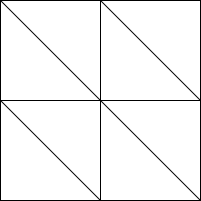
\includegraphics[width=1.0\linewidth,height=0.32\textheight,keepaspectratio]{data/synthetic_meshes/square_tesselation_2tri_Dirac_delta_1_v9_f8_wireframe.png}
		\caption{Sq2 v9\_f8 wireframe}\label{fig:sq2.a}
	\end{subfigure}
	\begin{subfigure}[b]{0.48\linewidth}
		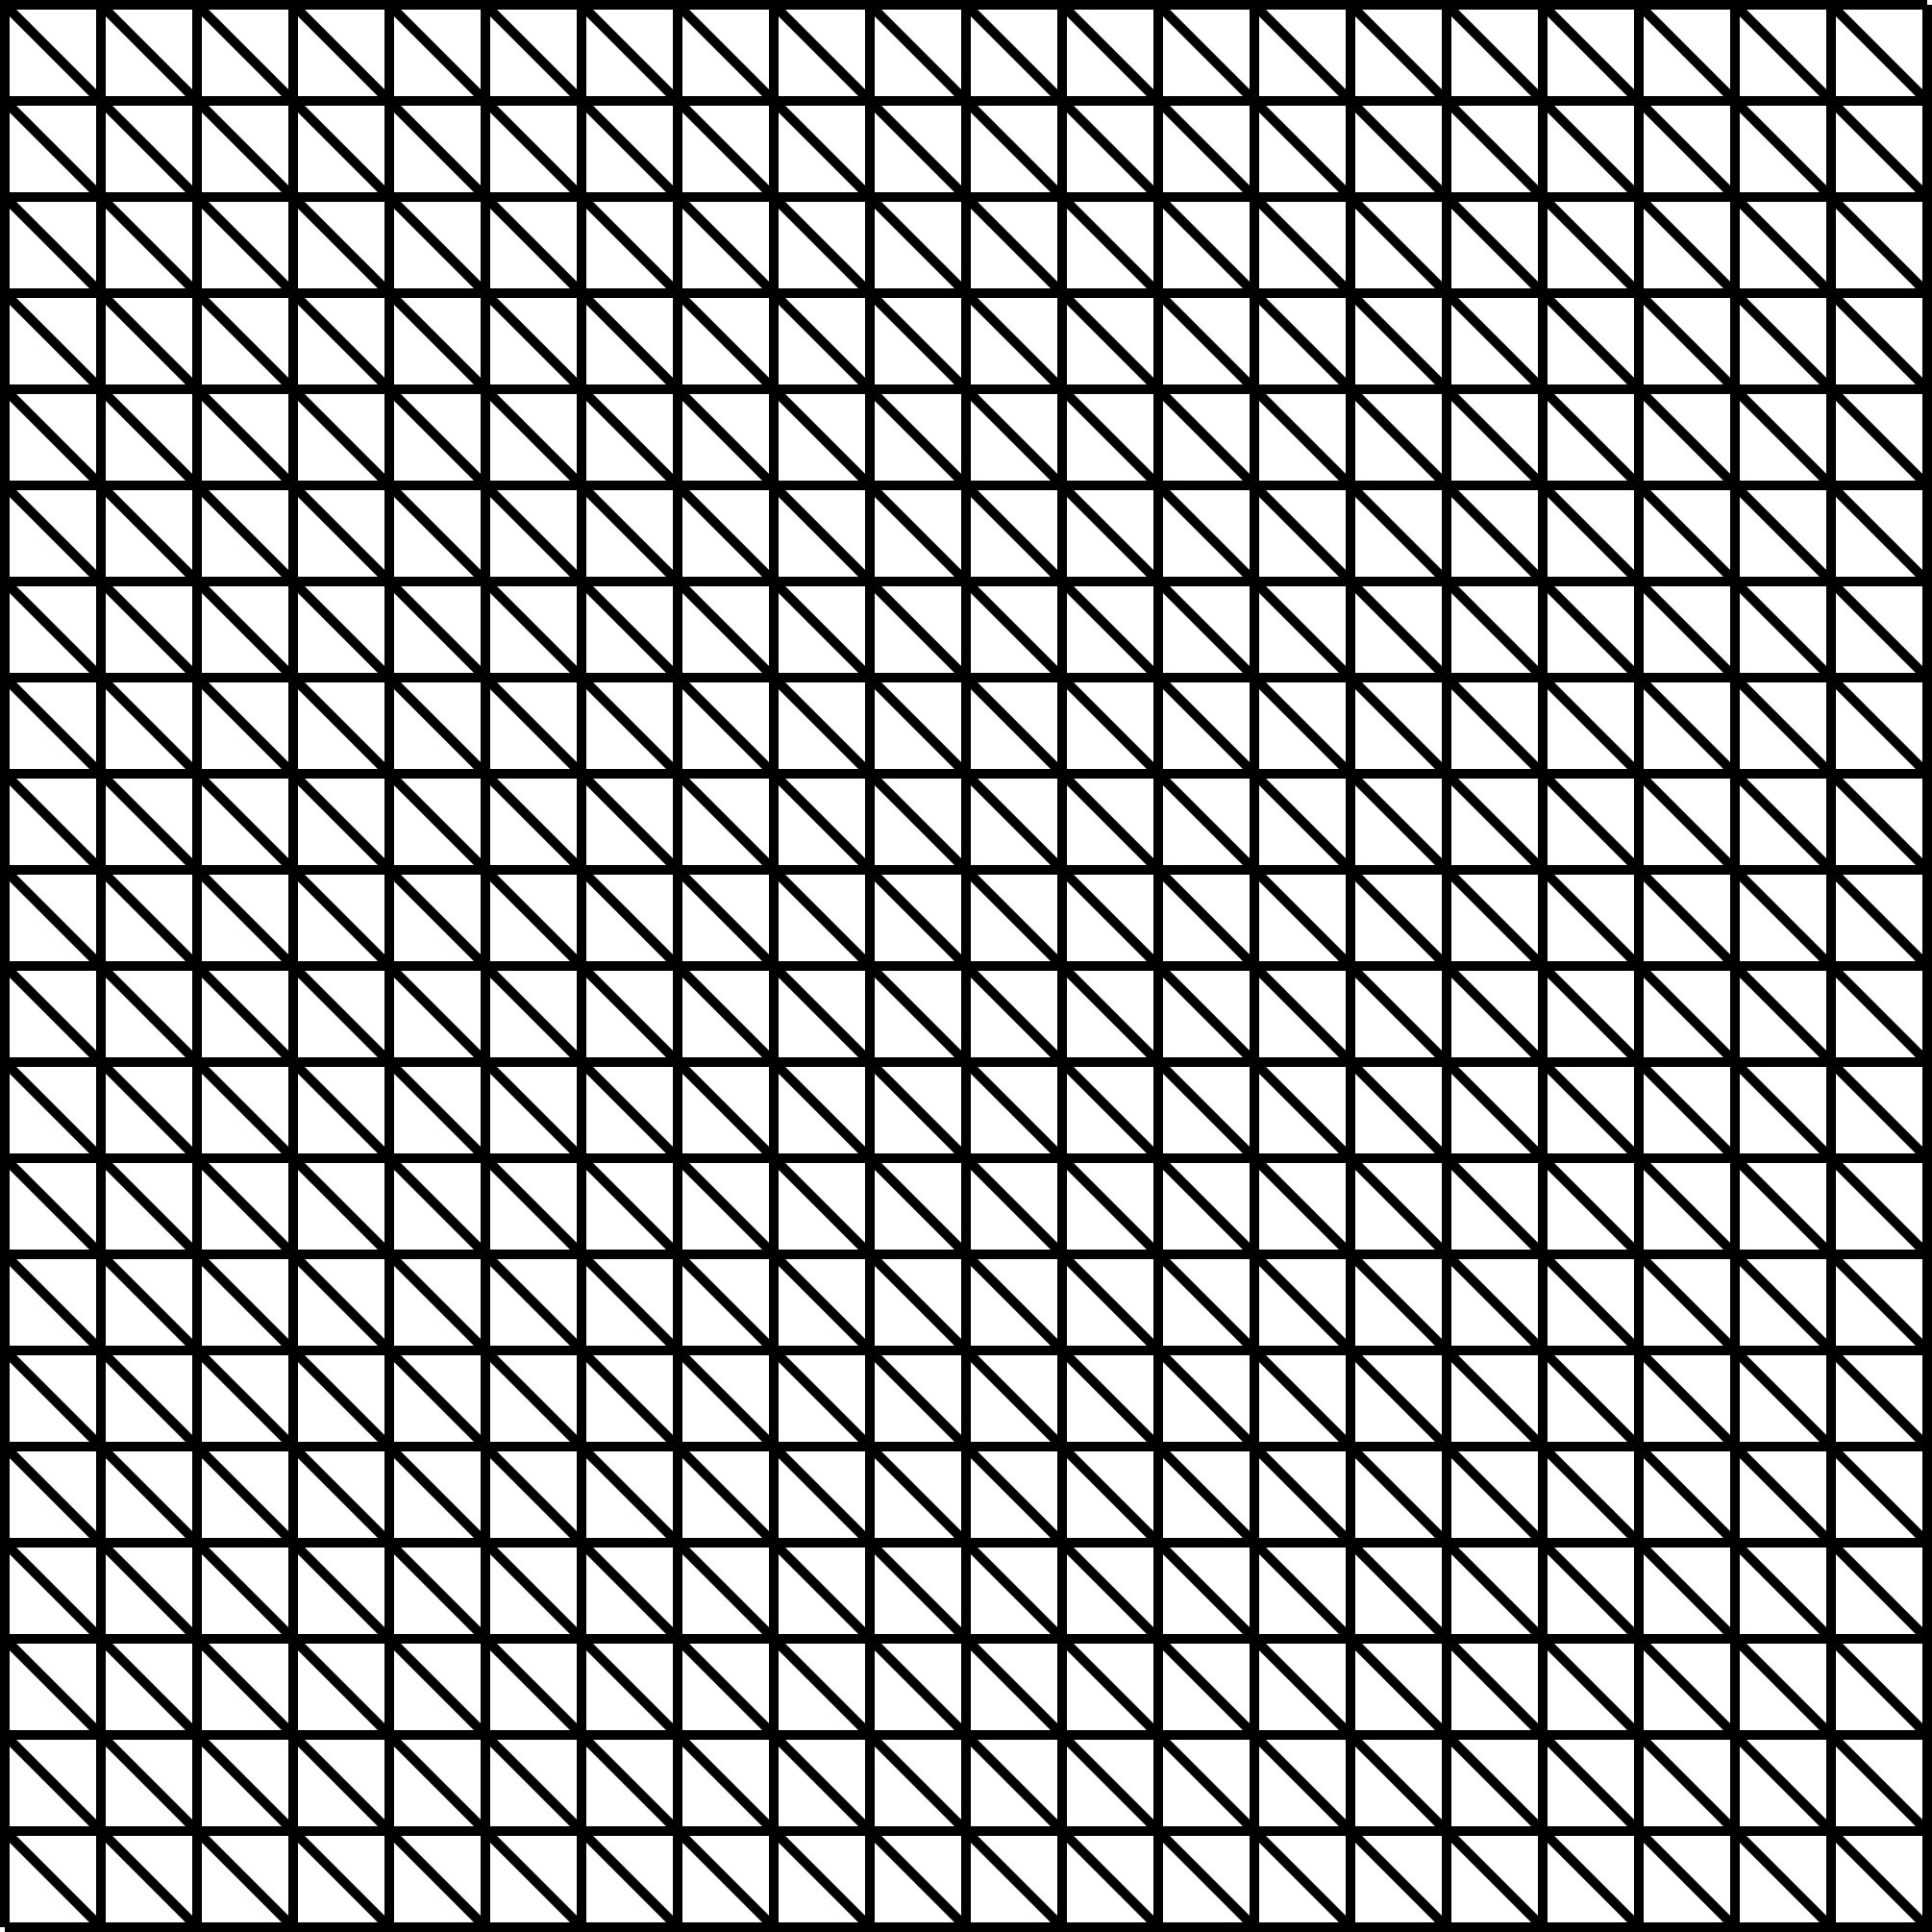
\includegraphics[width=1.0\linewidth,height=0.32\textheight,keepaspectratio]{data/synthetic_meshes/square_tesselation_2tri_Dirac_delta_10_v441_f800_wireframe.png}
		\caption{Sq2 v441\_f800 wireframe}\label{fig:sq2.b}
	\end{subfigure}

	\bigskip
	\begin{subfigure}[b]{0.48\linewidth}
		\includegraphics[width=1.0\linewidth,height=0.32\textheight,keepaspectratio]{data/synthetic_meshes/square_tesselation_2tri_Dirac_delta_1_v9_f8_funcvals_0iter_crop.png}
		\caption{Sq2 v9\_f8 iter 0}\label{fig:sq2.c}
	\end{subfigure}
	\begin{subfigure}[b]{0.48\linewidth}
		\includegraphics[width=1.0\linewidth,height=0.32\textheight,keepaspectratio]{data/synthetic_meshes/square_tessellation_2tri_Dirac_delta_10_v441_f800_funcvals_0iter.png}
		\caption{Sq2 v441\_f800 iter 0}\label{fig:sq2.d}
	\end{subfigure}

	\bigskip
	\begin{subfigure}[b]{0.48\linewidth}
		\includegraphics[width=1.0\linewidth,height=0.32\textheight,keepaspectratio]{data/synthetic_meshes/square_tesselation_2tri_Dirac_delta_1_v9_f8_funcvals_1iter_crop.png}
		\caption{Sq2 v9\_f8 iter 1}\label{fig:sq2.e}
	\end{subfigure}
	\begin{subfigure}[b]{0.48\linewidth}
		\includegraphics[width=1.0\linewidth,height=0.32\textheight,keepaspectratio]{data/synthetic_meshes/square_tessellation_2tri_Dirac_delta_10_v441_f800_funcvals_100iter.png}
		\caption{Sq2 v441\_f800 iter 100}\label{fig:sq2.f}
	\end{subfigure}}
	{\caption[Synthetic Square, 2 triangles, Dirac delta function]{A synthetic square, subdivided by triangles, with a Dirac delta function applied: (a) wireframe (b) colored by function value before filter (c) colored by function value after 1000 iterations
%GigaMesh~\cite{Mara10} with function values colored with the Improved Hot colorramp, exported as png after disabling the background grid [f7], maximizing the window, disabling screenshot cropping, as well as rejecting tiled rendering, finally cropping to content in GIMP.
	}\label{fig:sq2}}
\end{figure}
\todoCitation
\todoResearch{Why does sq2 10 need 100 iters to match sq 1 at 1 iters?}
\todoStyle{Why does sq2 1 iters 0 get differnt spacing?}
\todoStyle{Adjusting height, shrinks width => images no longer centered in their columns}

\subsubsection{Square grid, four triangles}

\subsubsection{Hexagonal grid}
\begin{figure}[ht]
\ffigbox
	{\begin{subfigure}[b]{0.48\linewidth}
		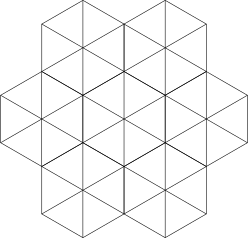
\includegraphics[width=1.0\linewidth,height=0.3\textheight,keepaspectratio]{data/synthetic_meshes/hexagonal_tessellation_Dirac_delta_1_v31_f42_wireframe.png}
		\caption{Hex v31\_f42 wireframe}\label{fig:hex.a}
	\end{subfigure}
	\begin{subfigure}[b]{0.48\linewidth}
		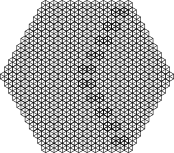
\includegraphics[width=1.0\linewidth,height=0.3\textheight,keepaspectratio]{data/synthetic_meshes/hexagonal_tessellation_Dirac_delta_10_v1057_f1986_wireframe.png}
		\caption{Hex v1057\_f1986 wireframe}\label{fig:hex.b}
	\end{subfigure}

	\bigskip
	\begin{subfigure}[b]{0.48\linewidth}
		\includegraphics[width=1.0\linewidth,height=0.3\textheight,keepaspectratio]{data/synthetic_meshes/hexagonal_tessellation_Dirac_delta_1_v31_f42_funcvals_0iter_crop.png}
		\caption{Hex v31\_f42 iter 0}\label{fig:hex.c}
	\end{subfigure}
	\begin{subfigure}[b]{0.48\linewidth}
		\includegraphics[width=1.0\linewidth,height=0.3\textheight,keepaspectratio]{data/synthetic_meshes/hexagonal_tessellation_Dirac_delta_10_v1057_f1986_funcvals_0iter_crop.png}
		\caption{Hex v1057\_f1986 iter 0}\label{fig:hex.d}
	\end{subfigure}

	\bigskip
	\begin{subfigure}[b]{0.48\linewidth}
		\includegraphics[width=1.0\linewidth,height=0.3\textheight,keepaspectratio]{data/synthetic_meshes/hexagonal_tessellation_Dirac_delta_1_v31_f42_funcvals_2iter_crop.png}
		\caption{Hex v31\_f42 iter 2}\label{fig:hex.e}
	\end{subfigure}
	\begin{subfigure}[b]{0.48\linewidth}
		\includegraphics[width=1.0\linewidth,height=0.3\textheight,keepaspectratio]{data/synthetic_meshes/hexagonal_tessellation_Dirac_delta_10_v1057_f1986_funcvals_200iter_crop.png}
		\caption{Hex v1057\_f1986 iter 200}\label{fig:hex.f}
	\end{subfigure}}
	{\caption[Synthetic Hexagonal Tessellations, Dirac delta function]{A synthetic hexagonal tessellation, subdivided by triangles, with a Dirac delta function applied: (a) v31 f42 wireframe (b) v1057 f1986 wireframe (c) v31 f42 colored by function value before filter (d) v1057 f1986 colored by function value before filter (e) v31 f42 colored by function value after 2 iterations (e) v1057 f1986 colored by function value after 200 iterations. 
% All using the colorramp "Hot (improved)"~\cite[p.~???]{Brewer2003}~\cite[p.~19]{Giga17}, visualized using GigaMesh~\cite{Mara10}, exported as png after disabling the background grid [f7], maximizing the window, disabling screenshot cropping, as well as rejecting tiled rendering, finally cropping to content in GIMP.
	}\label{fig:hex}}
\end{figure}
\todoCitation

\subsubsection{Random vertices within a circle}
\begin{figure}[ht]
\ffigbox
	{\begin{subfigure}[b]{0.48\linewidth}
		\includegraphics[width=1.0\linewidth,height=0.3\textheight,keepaspectratio]{data/synthetic_meshes/random_circle_tessellation_Dirac_delta_1_v11_f12_wireframe.png}
		\caption{R.Circ v11\_f12 wireframe}\label{fig:rcirc.a}
	\end{subfigure}
	\begin{subfigure}[b]{0.48\linewidth}
		\includegraphics[width=1.0\linewidth,height=0.3\textheight,keepaspectratio]{data/synthetic_meshes/random_circle_tessellation_Dirac_delta_10_v641_f1252_wireframe.png}
		\caption{R.Circ v641\_f1252 wireframe}\label{fig:rcirc.b}
	\end{subfigure}

	\bigskip
	\begin{subfigure}[b]{0.48\linewidth}
		\includegraphics[width=1.0\linewidth,height=0.3\textheight,keepaspectratio]{data/synthetic_meshes/random_circle_tessellation_Dirac_delta_1_v11_f12_funcvals_0iter.png}
		\caption{R.Circ v11\_f12 iter 0}\label{fig:rcirc.c}
	\end{subfigure}
	\begin{subfigure}[b]{0.48\linewidth}
		\includegraphics[width=1.0\linewidth,height=0.3\textheight,keepaspectratio]{data/synthetic_meshes/random_circle_tessellation_Dirac_delta_10_v641_f1252_funcvals_0iter.png}
		\caption{R.Circ v641\_f1252 iter 0}\label{fig:rcirc.d}
	\end{subfigure}

	\bigskip
	\begin{subfigure}[b]{0.48\linewidth}
		\includegraphics[width=1.0\linewidth,height=0.3\textheight,keepaspectratio,height=0.3\textheight,keepaspectratio]{data/synthetic_meshes/random_circle_tessellation_Dirac_delta_1_v11_f12_funcvals_0iter.png}
		\caption{R.Circ v11\_f12 iter 2}\label{fig:rcirc.e}
	\end{subfigure}
	\begin{subfigure}[b]{0.48\linewidth}
		\includegraphics[width=1.0\linewidth,height=0.3\textheight,keepaspectratio,height=0.3\textheight,keepaspectratio]{data/synthetic_meshes/random_circle_tessellation_Dirac_delta_10_v641_f1252_funcvals_10000iter.png}
		\caption{R.Circ v641\_f1252 iter 10,000}\label{fig:rcirc.f}
	\end{subfigure}}
	{\caption[Synthetic random vertices equally distributed per radius, Dirac delta function]{A synthetic circle filled with random vertices equaly distributed per radius, triangulated by Delauney method~\cite[p.~??]{todoCitation}, with a Dirac delta function applied: (a) v11\_f12 wireframe (b) v641\_f1252 wireframe (c) v11\_f12 colored by function value before filter (d) v641\_f1252 colored by function value before filter (e) v11\_f12 colored by function value after 2 iterations (f) v641\_f1252 colored by function value after 10,000 iterations. 
%All using the colorramp "Hot (improved)"~\cite[p.~???]{Brewer2003}~\cite[p.~19]{Giga17}, visualized using GigaMesh~\cite{Mara10}, exported as png after disabling the background grid [f7], maximizing the window, disabling screenshot cropping, as well as rejecting tiled rendering, finally cropping to content in GIMP.
}\label{fig:rcirc}}
\end{figure}
\todoCitation 
\todoResearch{Why and who equally distributed}

%\subsection{Debossed H}
%In Figure \ref{fig:h}, we show a debossed capital letter H.\footnote{The H is 
%as a nod to Heidelberg University and the cuniform script studied by the FCGL.}
%\begin{figure}[ht]
%\centering
%	\begin{subfigure}{.48\linewidth}
%		\centering
%		\resizebox{0.48\linewidth}{!}{\input{data/synthetic_meshes/h.tikz_labels.tex}}
%		\caption{HWireframe}\label{fig:h.a}
%	\end{subfigure}
%	\hfill
%	\begin{subfigure}{.48\linewidth}
%		\centering
%		\includegraphics[width=0.48\linewidth]{data/synthetic_meshes/h_colored.png}
%		\caption{HColored}\label{fig:h.b}
%	\end{subfigure}
%	\caption[A debossed H, which contains 22 vertices and 36 faces.]{A debossed H, 
%	which contains 22 vertices and 36 faces: (a) wireframe (b) colored by the 
%	relation to its distance to an underlying plane, in RdGy 
%	colorramp~\cite[p.~???]{Brewer2003}~\cite[p.~19]{Giga17}, visualized using the 
%	GigaMesh~\cite{Mara10} framework with triangle edges rendered.}\label{fig:h}
%\end{figure}
To evaluate methods available for discrete surfaces, we can increase the number 
of vertices of our synthetic wedge using five iterations of the mid-edge 
subdivision scheme [PR97,
HW99].~\cite[p.~38]{Mara12}



\section{Acquired Data}
Acquired Data examples are actually recorded by sensors.
Something in Archaeology
Cuneiform Tablets
Mayan Tablets
Dynamic Earth models

\subsection{University Seal}
Unisiegel\_\- UAH\_\- Ebay-Siegel\_\- Uniarchiv\_\- HE2066-60\_\- 010614\_\- partial\_\- ASCII.ply

\subsection{Mars Crater}
Mars dataset crater as a Digital Terrain Models (DTMs) Mention in Mara 3.6 
Summary “Dali” inspired methodProcessing regular grids like Digital Terrain 
Models (DTMs) will gain dramatic performance increases using the estimator, 
while processing irregular grids with high curvatures will strongly benefit 
from precise computation of the volume integral invariant.~\cite[p.~143]{Mara12}

\subsection{A Flat surface}
Flat surfaces have NOISE!

\subsection{Stanford Bunny}
http://graphics.stanford.edu/data/3Dscanrep/ (Stanford Bunny)



\section{Evaluation}
\subsection{Compute Times}

\begin{figure}[ht]
	\centering
	\includegraphics[width=1.0\linewidth,height=1.0\textheight,keepaspectratio]{plots/computeTimesLinespoints.png}
	\RawCaption{\caption[Compute Times - Linespoints]{Compute Times of Applying
		the	One-Ring Filter for Selected Numbers of Iterations onto Acquired and 
		Synthetic 3D Meshes of Varying Sizes}
		\label{fig:computeTimesLP}}
\end{figure}

\begin{figure}[ht]
	\centering
	\includegraphics[width=1.0\linewidth,height=1.0\textheight,keepaspectratio]{plots/computeTimesScatter.png}
	\RawCaption{\caption[Compute Times - Scatter]{Compute Times for Different
		Hardware Configurations by increaseing Mesh Size and Filter Iterations}
		\label{fig:computeTimesS}}
\end{figure}

\begin{figure}[ht]
	\centering
	\includegraphics[width=1.0\linewidth,height=1.0\textheight,keepaspectratio]{plots/numFacesByVerticesGoTo2.png}
	\RawCaption{\caption[Ratio of Faces / Vertices]{Ratio of Faces to Vertices by
		Increasing Vertex Count}
		\label{fig:ratioFacesVertices}}
\end{figure}





\section{Summary}
Lorem ipsum dolor sit amet, consectetur adipiscing elit. Morbi tincidunt eget 
ipsum eu iaculis. Cras vel sem eu velit eleifend porta vel sit amet massa. Etiam 
a posuere nunc. Aenean aliquam viverra dapibus. Aliquam ac eros a purus feugiat 
rhoncus. Donec faucibus ut nibh ut cursus. Aliquam erat volutpat. Proin efficitur 
nulla sit amet iaculis condimentum. Cras placerat leo vitae venenatis feugiat. In 
hac habitasse platea dictumst. Orci varius natoque penatibus et magnis dis 
parturient montes, nascetur ridiculus mus. In aliquet sagittis dui eu pulvinar. 
Morbi a arcu eu dolor sagittis varius. Aliquam dignissim tortor sed tortor 
suscipit, eget imperdiet mauris convallis.

\chapter{Distribution}
%CLI - commandline interface only
%Focus on theoretical work 
%And specifics regarding CUDA considerations regarding its limitations
%MAYBE 1 page
%Dependencies
%Linux vs Windows



\section{Standalone Precompiled Binary}
%CLI - commandline interface only

%\section[Acceleration by GPGPU]{Acceleration by General-purpose
%computing on Graphics Processing Units (GPGPU)}

\section{Integration with Legacy Code (GigaMesh)}
%CLI - commandline interface or GUI - graphical user interface are %possible
%\begin{enumerate}
%\item Make GigaMesh CUDA aware
%	\begin{enumerate}
%	\item Update Makefile to include nvcc compiler and new source files
%	\item second item
%	\end{enumerate}
%\item second item
%\end{enumerate}
%Before CUDA 5.0, if a programmer wanted to call particle::advance() from a CUDA kernel launched in main.cpp, the compiler required the main.cpp compilation unit to include the implementation of particle::advance() as well any subroutines it calls (v3::normalize() and v3::scramble() in this case). In complex C++ applications, the call chain may go deeper than the two-levels that our exampleillustrates. Without device object linking, the developer may need to deviate from the conventional application structure to accommodate this compiler requirement. Such changes are difficult for existing applications in which changing the structure is invasive and/or undesirable.~\cite{Cuda14}In order to use the full functionality of GigaMesh a batch program has to be run for generating feature vectors. These vectors contain additional information per vertex concerning surface and volume of a set of spheres intersecting the mesh. See [MKJB10] for more background information on the Multi Scale Integral Invariant (MSII) filtering technique. This operation is rather time consuming (it takes hours or even days of computing time) and therefore better runs without graphical user interface. Although generating feature vectors is quite robust against solo vertices, singularities, non-manifolds and holes, you should first clean up your mesh data to get a proper result. So switch to the advanced task of polishing your mesh in section 4.1 and return to this section when you have got a cleaned mesh. If you do not want to manipulate your mesh you may continue directly. Open a terminal and type and change to the mesh-folder by typing cd GigaMesh/mesh (note that GigaMesh stands for the GigaMesh installation folder). Then start the program nohup ./meshgeneratorfeaturevectors25d\_threads -f [-r 2] \& and use nohup at the beginning of the command and \& at the end to ensure that the job runs in the background. This is because this step can take several hours and you do not want to block the terminal.~\cite[p.~19]{Giga17}



\section{Summary}
%

\chapter{Conclusions}
As of this writing, the fastest available GPGPU card available is the Quadro RTX 6000 which has 4,608 parallel processing cores and can perform at 16.3 TFLOPS~\cite{quadro6k}, up from the the previous 5000 model, which already had 3,702 and could perform at 11.2 TFLOPS~\cite{quadro5k}.

%
%
%
%
\subsubsection{Summary}

%
%
%
%
\section{Future Work}
What they are and why I did not.
\begin{itemize}
	\item Implement in OpenCL to include all GPUs
	\item Implement in OpenMP to use multiple machines
	\item Implement in PThreads to exploit MIMP
	\item Pipelining memory reads/calculations exploit more concurrency
	\item Edge case handling: max mesh size in memory, Derive calculation for compute time per iteration by mesh size. Maybe find when load time is greater than iteration time
	\item support other file types
	\item Calculating edge length takes longest, so DO NOT DOUBLE EFFORT HERE
	\item Determine is using $\elm$ vs $\bar{\elm}$ has any effect, especially on one-ring neighborhood with a relatively large $\elm$ on mesh with a very small $\bar{\elm}$
	\item More analysis on \fors. it is my intuition that the un-isotropic nature of the filter is due to the speed at which information travels along longer edges.
	\item Apply the filter to multi-channel vector fields like RGB, however color-wheel based methods may be better
	\item Implement Median and Mode version of filter (others based on what's foudn in 2d filter results)
	\item Implement more storage vs speed options
	\item explore using the inner angles $\alpha_i$ in stead of area for weighting
	\item instead of global min size, just choose a size, especially if not using sqrt to get edgelengths
\end{itemize}


%
\appendix
\include{chapters/A1-Appendix}
\include{chapters/A2-Appendix}
%
\backmatter
\printindex
\printglossaries
\bibliography{thesis}{}
\bibliographystyle{plain}
\todoRemove{remove todoCitation from bibliography}
\todoStyle{should bibliographystyle be plain?}

\end{document}

